% SIAM Article Template
\documentclass[review,onefignum,onetabnum]{siamart171218}
\usepackage{booktabs}
\usepackage{graphicx,epstopdf} 
\usepackage[caption=false]{subfig} 
\usepackage{braket,amsfonts,amsopn} % <- Preamble
\usepackage{algorithmic}
 \Crefname{ALC@unique}{Line}{Lines}
 \usepackage{multirow}
\usepackage{xspace} 
\usepackage{comment}
\usepackage{siunitx} 
\usepackage{amssymb}


\definecolor{amber}{rgb}{1.0, 0.49, 0.0}
\definecolor{carmine}{rgb}{0.59, 0.0, 0.09}

\newenvironment{conditions}
{\par\vspace{\abovedisplayskip}\noindent\begin{tabular}{>{$}l<{$} @{${}={}$} l}}
	{\end{tabular}\par\vspace{\belowdisplayskip}}

% Information that is shared between the article and the supplement
% (title and author information, macros, packages, etc.) goes into
% ex_shared.tex. If there is no supplement, this file can be included
% directly.

% SIAM Shared Information Template
% This is information that is shared between the main document and any
% supplement. If no supplement is required, then this information can
% be included directly in the main document.


% Packages and macros go here
\usepackage{lipsum}
\usepackage{amsfonts}
\usepackage{graphicx}
\usepackage{epstopdf}
\usepackage{algorithmic}
\ifpdf
  \DeclareGraphicsExtensions{.eps,.pdf,.png,.jpg}
\else
  \DeclareGraphicsExtensions{.eps}
\fi

% Add a serial/Oxford comma by default.
\newcommand{\creflastconjunction}{, and~}

% Used for creating new theorem and remark environments
\newsiamremark{remark}{Remark}
\newsiamremark{hypothesis}{Hypothesis}
\crefname{hypothesis}{Hypothesis}{Hypotheses}
\newsiamthm{claim}{Claim}

% Sets running headers as well as PDF title and authors
\headers{RACE}{Christie Louis Alappat}

% Title. If the supplement option is on, then "Supplementary Material"
% is automatically inserted before the title.
\title{RACE\thanks{Submitted to the editors DATE.
\funding{This work was funded by the Fog Research Institute under contract no.~FRI-454.}}}

% Authors: full names plus addresses.
%\author{Christie Louis Alappat\thanks{FAU, Erlangen
%  (\email{christie.alappat@fau.de}).}
%\and X \thanks{Department of Applied Mathematics, Fictional University, Boise, ID 
%  (\email{X.edu}, \email{X@fictional.edu}).}
%\and Y\footnotemark[3]}

\usepackage{amsopn}
\DeclareMathOperator{\diag}{diag}


%%% Local Variables: 
%%% mode:latex
%%% TeX-master: "ex_article"
%%% End: 


% Optional PDF information
\ifpdf
\hypersetup{
  pdftitle={RACE},
  pdfauthor={}
}
\fi

% The next statement enables references to information in the
% supplement. See the xr-hyperref package for details.

%\externaldocument{ex_supplement}

% FundRef data to be entered by SIAM
%<funding-group>
%<award-group>
%<funding-source>
%<named-content content-type="funder-name"> 
%</named-content> 
%<named-content content-type="funder-identifier"> 
%</named-content>
%</funding-source>
%<award-id> </award-id>
%</award-group>
%</funding-group>

\def\GW{\color{blue}}
\def\CA{\color{red}}

\newcommand{\RAC}{RAC\xspace}
\newcommand{\RACfull}{Recursive Algebraic Coloring\xspace}
\newcommand{\RACfullNoSpace}{Recursive Algebraic Coloring}
\newcommand{\RACE}{RACE \xspace}
\newcommand{\RACEfull}{Recursive Algebraic Coloring Engine\xspace}
\newcommand{\DONE}{distance-$1$\xspace}
\newcommand{\DTWO}{distance-$2$\xspace}
\newcommand{\DK}{distance-$k$\xspace}
\newcommand{\etal}{et al.\xspace}
\newcommand{\RSB}{RSB\xspace}
\newcommand{\SpMV}{SpMV\xspace}
\newcommand{\SymmSpmv}{SymmSpMV\xspace}
\newcommand{\SpMTV}{SpMTV\xspace}
\newcommand{\GS}{GS\xspace}
\newcommand{\SYMMGS}{SymmGS\xspace}
\newcommand{\KACZ}{KACZ\xspace}
\newcommand{\SYMMKACZ}{SymmKACZ\xspace}
\newcommand{\Intel}{Intel\xspace}
\newcommand{\AMD}{AMD\xspace} 
\newcommand{\IVB}{Ivy-Bridge\xspace}
\newcommand{\BDW}{Broadwell\xspace}
\newcommand{\SKX}{Skylake\xspace}
\newcommand{\NAP}{Naples\xspace}
\newcommand{\EPY}{Epyc\xspace}
\newcommand{\CRS}{CRS\xspace}
\newcommand{\CRSfull}{Compressed Row Storage\xspace}
\newcommand{\MC}{MC\xspace}
\newcommand{\MCfull}{multi-coloring\xspace}
\newcommand{\ABMC}{ABMC\xspace}
\newcommand{\ABMCfull}{algebraic block multi-coloring\xspace}
\newcommand{\NNZR}{$N_{nzr}$\xspace}
\newcommand{\NNZRSYMM}{$N_{nzr}^{symm}$\xspace}
\newcommand{\NNZRmath}{N_{nzr}\xspace}
\newcommand{\NNZRmathSYMM}{N_{nzr}^{symm}\xspace}
\newcommand{\LIKWID}{LIKWID\xspace}
\newcommand{\likwidBench}{$likwid-bench$\xspace}
\newcommand{\LLC}{LLC\xspace}
\newcommand{\LLCfull}{last level cache\xspace}
\newcommand{\ie}{i.e.,\xspace}
\newcommand{\cf}{cf. \xspace}
\newcommand{\ESSEX}{ESSEX\xspace}
\newcommand{\LCCfull}{Low Core Count\xspace}
\newcommand{\LCC}{LCC\xspace}
\newcommand{\HCCfull}{High Core Count\xspace}
\newcommand{\HCC}{HCC\xspace}
\newcommand{\MB}{MB\xspace}
\newcommand{\KB}{kB\xspace}
\newcommand{\GB}{GB\xspace}
\newcommand{\TB}{TB\xspace}
\newcommand{\SIMD}{SIMD\xspace}
\newcommand{\RCMfull}{Reverse Cuthill McKee\xspace}
\newcommand{\RCM}{RCM\xspace}
\newcommand{\CMfull}{Cuthill McKee\xspace}
\newcommand{\BFSfull}{Breadth First Search\xspace}
\newcommand{\BFS}{BFS\xspace}
\newcommand{\CPU}{CPU\xspace}
\newcommand{\pt}{pt.\xspace}
\newcommand{\Stex}{Stencil example\xspace}
\newcommand{\stex}{stencil example\xspace}
\newcommand{\Inorder}{In order\xspace}
\newcommand{\inorder}{in order\xspace}
\newcommand{\levelPtr}{{\tt level\_ptr}\xspace}
\newcommand{\atleast}{at least\xspace}
\newcommand{\totalLvl}{$n_l$\xspace}
\newcommand{\totalLvlMATH}{n_l}
\newcommand{\level}{level\xspace}
\newcommand{\levels}{levels\xspace}
\newcommand{\levelGroup}{level group\xspace}
\newcommand{\levelGroups}{level groups\xspace}
\newcommand{\LevelGroups}{Level groups\xspace}
\newcommand{\eg}{e.g.,\xspace}
\newcommand{\aka}{a.k.a.\xspace}
\newcommand{\subgraph}{sub-graph\xspace}
\newcommand{\subgraphs}{sub-graphs\xspace}
\newcommand{\levelTree}{{\tt level\_tree}\xspace}
\newcommand{\HPC}{HPC\xspace}
\newcommand{\effPar}{\emph{effective parallelism}\xspace}
\newcommand{\effRow}{\emph{effective row}\xspace}
\newcommand{\EffRow}{\emph{Effective row}\xspace}
\newcommand{\nthreads}{${n_{t}}$\xspace}
\newcommand{\nthreadsMath}{n_{t}\xspace}
\newcommand{\nrows}{${n_{r}}$\xspace}
\newcommand{\nrowsMath}{n_{r}\xspace}
\newcommand{\nrowsNospace}{${n_{r}}$}
\newcommand{\nnz}{${n_{nz}}$\xspace}
\newcommand{\nnzMath}{n_{nz}\xspace}
\newcommand{\nrowsEff}{${n_{r}^{eff}}$\xspace}
\newcommand{\nrowsEffMath}{n_{r}^{eff}\xspace}
\newcommand{\threadEff}{${n_{t}^{eff}}$\xspace}
\newcommand{\threadEffMath}{n_{t}^{eff}\xspace}
\newcommand{\upto}{up to \xspace}
\newcommand{\fracUnit}[2]{\Big[\frac{\mbox{#1}}{\mbox{#2}}\Big]}
\newcommand{\unit}[1]{\Big[\mbox{#1}\Big]}
\newcommand{\roofline}{roofline\xspace}
\newcommand{\METIS}{METIS\xspace}
\newcommand{\COLPACK}{COLPACK\xspace}
\newcommand{\SPMP}{Intel SpMP\xspace}
\newcommand{\MKL}{MKL\xspace}
\newcommand{\GF}{GF/s\xspace}
\newcommand{\SCAMACTfull}{Scalable Matrix Collection\xspace}
\newcommand{\SCAMACT}{ScaMac\xspace}
\begin{document}

\maketitle

% REQUIRED
\begin{abstract}
  % SIAM Shared Information Template
% This is information that is shared between the main document and any
% supplement. If no supplement is required, then this information can
% be included directly in the main document.
Many iterative numerical methods for sparse systems and important building blocks of sparse linear algebra feature strong data dependencies. These may be loop-carried dependencies as they occur in many iterative solvers or preconditioners (\eg of Gauss-Seidel (\GS) type) or write conflicts as they show up in the parallelization of building blocks such as symmetric sparse matrix vector multiplication (\SymmSpmv) or sparse matrix transpose vector multiplication (\SpMTV). Scalable, hardware-efficient parallelization of such kernels is known to be a hard problem in the general case of sparse matrices which do not have simple regular structures.

A standard approach to solve this problem is \MCfull (\MC) of the underlying matrix according to the requirements (\eg distance-1 for GS type iterations) of the algorithm. For irregular and/or large matrices this method may lead to load imbalance, frequent global synchronization and loss of data locality, which will reduce the single-node performance. These problems typically become more severe for higher order distance colorings and larger matrices. Among several improvement methods \ABMCfull (\ABMC) is the most promising for addressing those problems. However, \ABMC has been applied only for distance-1 coloring problems. These methods have in common that they do not take into account the requirements of modern hardware in terms of data locality, load balancing and degrees of parallelism available in modern compute nodes.

In this paper we present a novel recursive algebraic coloring approach solving general \DK dependencies. It is motivated by the shortcomings of existing \MC methods in terms of hardware efficiency and parallelization overhead. Our method addresses matrices with symmetric structure (but not necessarily symmetric matrix entries) and thus can be represented by an undirected graph. In a first step we do a \BFS pre-processing for bandwidth reduction of the graph, which aims to increase data locality for the underlying sparse matrix problems: Starting from a root vertex we construct the $levels$ of the \BFS algorithm \ie \level $i$ consists of all nodes having distance $i$ to the root vertex. We then permute the graph such that vertex numbering increases with distance from the root vertex. Coloring the resulting \levels would be a naive approach to generate a \DK coloring but would for obvious reasons (\eg \level 0 contains only one vertex) often lead to severe load imbalance. Thus we perform in a second step $level$ $aggregation$ of neighboring \levels, which aims at conserving data locality. The choice of the size of each \levelGroup is subject to two major constraints: First, for a \DK coloring of the original graph/problem at least $k$ \levels are aggregated into a \levelGroup (\aka $supernode$). This means that alternate \levelGroups can be executed in parallel which is equivalent to a \DONE coloring of the \levelGroups. Second, we apply a criterion for load balancing that considers the total amount of hardware threads to be used at execution time and tries to balance workload across these threads evenly. At this stage it might happen that most of the vertices end up in a few \levelGroups. Therefore, depending on the size of the \levelGroups, different number of threads will be assigned to each of them. \Inorder to further parallelize within this \levelGroup for assigned threads the entire procedure is recursively repeated on their corresponding \subgraphs subject to the \DK constraint. The aggregation step is controlled by a single external parameter which influences the load imbalance introduced by forming each \levelGroup. Due to the recursive nature of this algorithm, nested parallelism is required. However, only local synchronization is required between the threads assigned to the same \subgraph.

We have implemented our algorithm in the open source library \RACE (\RACEfull). \RACE  has two main usage scenarios: It can either return all relevant data structures and parallelization information required for manual implementation of the kernel at hand, or one can just use its callback function interface, which takes care of parallelization and all data handling automatically. As of now RACE is limited to shared memory nodes as it only supports thread-level parallelism. RACE uses the \CRSfull (\CRS) sparse matrix data format but can be easily extended to other formats.

Choosing a representative set of 28 sparse matrices we first perform an analysis of the impact of the aggregation parameter on the quality of the load balancing achieved for thread counts relevant for modern compute nodes. We observe that even for 60 threads, 70\% of the test matrices achieve more than 70\% of effective parallelism (theoretical efficiency) after accounting for load imbalances. This does not take into account scalability limitations like memory bandwidth bottleneck that occur in practice.

Finally we apply RACE to two iterative schemes which require \DONE (\GS solver) and \DTWO (Kaczmarz solver) as well as for parallel symmetric sparse matrix vector multiplication (\SymmSpmv)  (where \DTWO coloring is required to resolve write conflicts). We analyze \RACE performance and compare with \MC using \COLPACK, \ABMC using \COLPACK on top of \METIS, Intel \MKL if the kernel is available and data format (Recursive Sparse Blocks [RSB]) which is tailored for \SymmSpmv. Overall we achieve a speed-up of 2--2.5$\times$ compared to \MC and \MKL implementations. While we are on par with \ABMC for small matrices, for large matrices we gain almost a factor of 1.5--2$\times$. Comparisons with iterative kernels also highlight the convergence behavior of the method. Results show that the convergence of \RACE is better than \MC and is competitive with \ABMC.
\end{abstract}

% REQUIRED
\begin{keywords}
  example, \LaTeX
\end{keywords}

% REQUIRED
\begin{AMS}
  68Q25, 68R10, 68U05
\end{AMS}

\section{Key-Points in paper}
\begin{itemize}
	\item In this paper we propose a method to parallelize sparse linear algebra kernels having dependencies. The method is called \acrshort{RACE} and is a recursive level-based approach.  
	
	\item The main aim of the paper is to explain the \acrshort{RACE} method and procedures involved in it. Furthermore a brief parameter study and performance modeling of kernels executed with \acrshort{RACE} is carried out.
	
	\item In this paper we test our method for both \DONE (\acrshort{GS}) and \DTWO (\acrshort{SymmSpMV} and \acrshort{KACZ}) dependencies, and analyze both exact (\acrshort{SymmSpMV}) and iterative kernels (\acrshort{GS}, \acrshort{KACZ}).
	
	\item For \DONE kernels we compare against the existing approaches of \acrshort{MC} \cite{MC}, \acrshort{ABMC} \cite{ABMC} and \acrshort{MKL} \cite{MKL} implementations.
	
	\item For \DTWO kernels along with comparing against existing approaches of \acrshort{MC} \cite{feast_mc} and implementations in \acrshort{MKL} \cite{MKL}, we also extend the \acrshort{ABMC} method for \DTWO coloring. To our knowledge this is the first paper which uses \acrshort{ABMC} method for \DTWO coloring.
	
	\item Comparisons with \acrshort{SymmSpMV} (an exact kernel) enables us to solely study the performance behavior of \acrshort{RACE} compared with others, since here effects like convergence does not play a role. Overall we achieve a speed-up of $2-2.5 \times$ compared to \acrshort{MC} and \acrshort{MKL} implementations, while we are on par with \acrshort{ABMC} for small matrices and for large matrices we gain almost a factor of $1.5-2 \times$ benefit. 
	
	\item Comparisons with iterative kernels also puts into light the convergence behavior of the method. Results show that the convergence of \acrshort{RACE} is better than \acrshort{MC} and is competitive with \acrshort{ABMC} method.
	
	\item Finally we compare our method against a different sparse matrix data format known as \acrshort{RACE}, which is a tailored data format for working on kernels having dependencies. How much details on this comparison should we include in the paper? 
\end{itemize}

\section{Introduction}
The introduction introduces the context and summarizes the
manuscript. It is importantly to clearly state the contributions of
this piece of work. The next two paragraphs are text filler,
generated by the \texttt{lipsum} package.

A distance-$k$ coloring of a graph is an assignment of colors to vertices such that any two vertices connected by a path consisting of at most $k$ edges receive different colors, and the goal of the associated problem is to minimize the number of colors used.


% The outline is not required, but we show an example here.
The paper is organized as follows. Our main results are in
\cref{sec:main}, our new algorithm is in \cref{sec:alg}, experimental
results are in \cref{sec:experiments}, and the conclusions follow in
\cref{sec:conclusions}.


\section{Related Work}
\label{Sec:related_work}



% SIAM Shared Information Template
% This is information that is shared between the main document and any
% supplement. If no supplement is required, then this information can
% be included directly in the main document.
One of the earliest work on parallelizing kernels having loop-carried dependencies is the red-black Gauss-Seidel scheme \cite{RBGS}. Later Kamath and Sameh introduced a two-block partitioning scheme for parallelizing Kaczmarz method on tridiagonal structures \cite{Kamath}. A general study on the convergence of these block methods were done by Elfving in 1980 \cite{Elfving1980}.

The advent of processors having more parallelism and the need to consider more unstructured matrices have made graph-based approach an important tool for parallelizing such kernels. Multicoloring is one of the most popular approach used in this field \cite{MC}, but is sometimes not efficient on modern cache-based processors. There have been several researches going on to increase the efficiency of \MCfull and improving the heuristics, an overview of the methods can be found in \cite{equitable_color}. One of the most successful method in this regard is the \ABMCfull \cite{ABMC} proposed by Iwashita \etal in 2012. 

Another line of research focuses on parallelizing dependent kernels while maintaining the same convergence behavior of sequential execution. One of the earliest known works in this category is the hyperplane method \cite{saad} on FDM (Finite Difference Method) like matrices. Extensions to this approach can be seen in \cite{cm-rcm} where a hybrid approach between \MCfull and hyperplane method is used. However the most general method which falls into this category is level-scheduling \cite{saad}.  Efficient implementation of this method can be attributed to Park \etal with his work on triangular solvers \cite{park_ls}.

Most of the above mentioned method have been tested only for their applicability to parallelize \DONE dependent kernels and some of them are not capable to deal with dependencies like \DTWO. The research on parallelizing \DONE dependent kernels has been strongly accelerated after the introduction of HPCG benchmark \cite{hpcg}. When it comes to \DTWO kernels popular methods seen in the literature are locking based methods, thread private local vectors \cite{thread_private_symm_spmv,sparseX} for kernels like symmetric sparse matrix vector or with the usage of specially tailored sparse matrix data formats like compressed sparse blocks (CSB) \cite{CSB} or recursive sparse blocks (\RSB) \cite{RSB}.



\section{Contribution}
\label{Sec:contribution}
% SIAM Shared Information Template
% This is information that is shared \acrshort{ABMC} the main document and any
% supplement. If no supplement is required, then this information can
% be included directly in the main document.
The paper focuses on developing an alternative method to parallelize kernels having loop-carried dependencies. The method introduced here is applicable for solving general distance-k dependencies, similar to \acrfull{MC} methods. Currently we focus only on undirected graph \ie matrices with symmetric sparsity pattern (but not necessarily symmetric entries). The main motivation of the approach is to achieve good hardware performance on modern hardware architecture, by generating sufficient parallelism while preserving good data locality. The method needs no specialized data format, and works basically on simple sparse matrix format like \acrfull{CRS}.

Most of the above approaches explained above in \cref{Sec:related_work} suffer from performance penalties in one way or the other, for example \acrshort{MC} degrades the data locality, although this can be improved considerably using \acrfull{ABMC}, still for moderately large matrices or with the increase in $k$ of \DK dependency the method shows deterioration in performance. Similar drawbacks exists for other methods which will be discussed within this paper.

In this work we provide a detailed performance analysis of the method and comparison \acrshort{ABMC} different existing methods chosen from representative classes. The comparisons are done both for exact kernels like symmetric sparse matrix vector (\acrshort{SymmSpMV}) having \DTWO dependency and iterative solvers like \acrfull{KACZ}. For iterative scheme we further provide comparison \acrshort{ABMC} convergence of different methods. The comparisons are done on different hardware architectures ranging from Intel's \IVB series to modern \SKX architecture and the \AMD \EPY architecture. Here we also show the result of extension of \acrshort{ABMC} for \DTWO coloring which to our knowledge has not been studied previously. The comparisons shows the superiority of our method compared to others and the applicability of our method on wide-variety of heterogeneous systems. As far to our knowledge this is the first paper which demonstrates such high efficiency of \DTWO dependent kernels using simple and common \acrshort{CRS} matrix storage format on such broad scale of matrices.

The paper is limited to node level, and we use only thread level parallelization. Multi-node parallelization is left for future work. However it should be noted that for iterative kernels like \acrshort{KACZ} and \acrshort{GS} node-level performance is far more important because commonly such solvers are applied only locally and different approaches are used for parallelizing \acrshort{ABMC} nodes \cite{hpcg,CARP}.

\begin{comment}
As a final application run we demonstrate the parallelization of an eigen-value solver called FEAST \cite{FEAST}, where we use an iterative inner linear solver based on Kaczmarz method. The result presented is the first to achieve such high performance on node level for an iterative solver and is superior to the previous results published \cite{feast_mc}.
\end{comment}


\section{Test bed, matrices and kernels}
{\CA Need to change the name of the section}
\label{Sec:test_bed}
\subsection{Test bed}
{\GW ToDo: EPYC raus;}
The tests are conducted on two different multi-core architectures. One being Intel's \IVB and the other \SKX architecture, the choice of these architectures enable study of the method on two extreme generation of Intel's processor currently being used on \HPC systems. All the tests are conducted on a single socket (chip) of these architectures using all its available cores. 

\begin{itemize}
	\item \Intel \IVB architecture belongs to class of classic Intel's cache-based architecture, which has three inclusive cache  hierarchies. All the cache are scalable and the \LLC (L3) being shared among all the cores on one socket. The processor is capable of delivering one full four wide \SIMD add, multiply and load in one cycle. 
	\item \Intel \SKX architecture belongs to recent generation of Intel family. Contrary to it's predecessors (like \IVB), L3 cache is now changed to a non-inclusive victim cache shared by all the cores on a socket. The architecture comes with support for eight wide \SIMD operations (AVX-512). The processor is capable of doing two AVX-512 add, multiply and load operations per cycle.
	\begin{comment}
	\item {\GW \AMD \EPY is based on AMD's Zen microarchitecture. The basic building block of the architecture consists of Core Complex (CCX) consisting of three cores (can extend upto four on high end models) each having it's own private L1 and L2 cache. The L3 cache is shared between a core complex and is non-inclusive victim cache. A single socket of \EPY consists of eight such CCX.}
	\end{comment}
	
\end{itemize}
The details of architectures along with the measured bandwidths are given in \cref{tab:test_bed}. The bandwidths are measured using \likwidBench suite.

\begin{comment}
\begin{table}[tbhp]
\footnotesize
\caption{Compute node configurations. The last two columns present attainable bandwidth numbers ($b_S$) on a single socket, depending on the access pattern (copy vs. load only)}\label{tab:test_bed}
\begin{center}
%	\setlength{\tabcolsep}{3em}
	\begin{tabular}{|l| c  c c |}
		\toprule
		{Model name} & {Xeon\textsuperscript{\textregistered} E5-2660} & {Xeon\textsuperscript{\textregistered} Gold 6148} & { Epyc 7451 } \\
		\midrule
		{Microarchitecture} & {Ivy Bridge} & {Skylake} & {Zen} \\
		\midrule
		{Clock} & {2.2 GHz} & {2.4 GHz} & {2.3 GHz}\\
		{Physical Cores per socket} & {10} & {20} & {24}\\
		{L1d Cache} & {10 $\times$ 32 \KB} & {20 $\times$ 32 \KB} & {24 $\times$  32 \KB}\\
		{L2 Cache} & {10 $\times$ 256 \KB} & {20 $\times$ 1 \MB} & {24 $\times$ 512 \MB }\\
		{L3 Cache} & {25 \MB} & {27.5 \MB} & {8 $\times$ 8 \MB}\\
		{L3 type} & {inclusive} & {non-inclusive} & {non-inclusive}\\
		{Main Memory} & {32 GB} & {45 GB} & {4 $\times$ 16 GB}\\
		{Bandwidth per socket - load only} & {47 GB/s} & {115 GB/s} & {130 GB/s }\\ %TODO
		{Bandwidth per socket - copy} & {40 GB/s} & {104 GB/s} & {114 GB/s }\\
		\bottomrule
	\end{tabular}
\end{center}
\end{table} 
\end{comment}

\begin{table}[tbhp]
	\footnotesize
	\caption{Test bed}\label{tab:test_bed}
	\begin{center}
		%	\setlength{\tabcolsep}{3em}
		\begin{tabular}{|l| c  c |}
			\toprule
			{Model name} & {Xeon\textsuperscript{\textregistered} E5-2660} & {Xeon\textsuperscript{\textregistered} Gold 6148} \\
			\midrule
			{Microarchitecture} & {Ivy Bridge} & {Skylake} \\
			\midrule
			{Clock} & {2.2 GHz} & {2.4 GHz}\\
			{Physical Cores per socket} & {10} & {20} \\
			{L1d Cache} & {10 $\times$ 32 \KB} & {20 $\times$ 32 \KB}\\
			{L2 Cache} & {10 $\times$ 256 \KB} & {20 $\times$ 1 \MB} \\
			{L3 Cache} & {25 \MB} & {27.5 \MB}\\
			{L3 type} & {inclusive} & {non-inclusive}\\
			{Main Memory} & {32 GB} & {45 GB}\\
			{Bandwidth per socket - load only} & {47 GB/s} & {115 GB/s}\\ %TODO
			{Bandwidth per socket - copy} & {40 GB/s} & {104 GB/s}\\
			\bottomrule
		\end{tabular}
	\end{center}
\end{table} 

Furthermore all the measurements were done with  \CPU clock speeds fixed at frequencies indicated in \cref{tab:test_bed}.


\subsection{External Tools and Software}
Following external libraries are used in this paper. The application of these libraries will be stated at the point it is needed.
\begin{itemize}
	%TODO
	\item \LIKWID \cite{LIKWID} \text{\tt{likwid-perfctr}} is used for measuring hardware performance counters and \text{\tt{likwid-bench}}  for measuring bandwidth.
	\item \COLPACK \cite{COLPACK} is used for pre-processing matrix by \MCfull.
	\item \SPMP \cite{SpMP} is used to perform \RCMfull (\RCM).
	\item \METIS\cite{METIS} is used for graph partitioning in \ABMC approach.
	\item All the code used was compiled with Intel compiler version 17.0.3 and the following compiler flags were set {\tt -fno-alias -xHost -O3} for Ivy-Bridge system and {\tt -fno-alias -xCORE-AVX512 -O3} for Skylake system.
	\item \MKL \cite{MKL} version 17 is used for performing some reference sparse matrix computations.
\end{itemize}

\subsection{Benchmark Matrices}
All the test matrices are taken from SuiteSparse Matrix Collection (former University of Florida Sparse Matrix Collection) \cite{UOF} and quantum physics field (see \ESSEX project \cite{ESSEX} for more details). The selection of the matrices from SuiteSparse Matrix Collection is  mainly done by combining the test matrices from two papers \cite{RSB,park_ls}. This enables easy comparison of results. Matrices from \ESSEX project are some of the matrices that are of interest in the iterative FEAST eigen value solver that internally uses Kaczmarz solver, these matrices can be generated using \SCAMACTfull open source library (\SCAMACT).{\CA but Graphene not} %TODO cite SCAMACT
  Only matrices having undirected graphs are considered due to scope of the paper as mentioned in \cref{Sec:contribution}. Matrices along with some of their parameters are given in \cref{table:bench_matrices}.  Matrices that have been marked with an * symbol indicate they are corner cases and will be discussed in detail.

\begin{table}[ht]
	\footnotesize
	\caption{Details of benchmark matrices. Matrices with an * symbol in the column `C' indicates that they are chosen corner cases. Column `S' shows the source of the matrix, matrix without any label indicates they come from SuiteSparse Matrix Collection and one marked with * indicate they come from \SCAMACT matrix collection. {\CA maybe it's better to mention ESSEX since Graphene cannot be generated with SCAMACT} }\label{tab:test_mtx}
	\label{table:bench_matrices}
	\begin{center}
			\begin{tabular}{|l|l|c|c|c|c|c|}
		\toprule
		{Index} & {Matrix name} & {nrows} & {nnz} & {bandwidth} &  {} &  \\
		\midrule
{1}	& {audikw\_1}	& {943695}	& {77651847}	& {925946}	& {} & \multirow{24}{*}{\rotatebox[origin=c]{90}{SuiteSparse Matrix Collection}}\\
{2}	& {bone010}	& {986703}	& {71666325}	& {13016}	& {} & \\
{3}	& {channel-500x100x100-b050}	& {4802000}	& {85362744}	& {600299} & {} &	\\
{4}	& {crankseg\_1}	& {52804}	& {10614210}	& {50388} &	{*} & \\
{5}	& {delaunay\_n24}	& {16777216}	& {100663202}	& {16769102}	& {} & \\
{6}	& {dielFilterV3real}	& {1102824}	& {89306020}	& {1036475}	& {} &\\
{7}	& {Emilia\_923}	& {923136}	& {41005206}	& {17279}	& {} &\\
{8}	& {F1}	& {343791}	& {26837113}	& {343754}	& {} & \\
{9}	& {Fault\_639}	& {638802}	& {28614564}	& {19988}	& {} & \\
{10}	& {Flan\_1565}	& {1564794}	& {117406044}	& {20702}	& {} & \\
{11}	& {G3\_circuit}	& {1585478}	& {7660826}	& {947128}	& {} & \\
{12}	& {Geo\_1438}	& {1437960}	& {63156690}	& {26018}	& {} & \\
{13}	& {gsm\_106857}	& {589446}	& {21758924}	& {588744}	& {} & \\
{14}	& {Hook\_1498}	& {1498023}	& {60917445}	& {29036}	& {} & \\
{15}	& {HPCG-192}	& {7077888}	& {189119224}	& {37057}	& {} & \\
{16}	& {inline\_1}	& {503712}	& {36816342}	& {502403}	& {} & \\
{17}	& {nlpkkt120}	& {3542400}	& {96845792}	& {1814521} &  & \\
{18}	& {nlpkkt200}	& {16240000}	& {448225632}	& {8240201}	& {*} & \\
{19}	& {offshore}	& {259789}	& {4242673}	& {237738}	& {*} & \\
{20}	& {parabolic\_fem}	& {525825}	& {3674625}	& {525820}	& {*} & \\
{21}	& {pwtk}	& {217918}	& {11634424}	& {189331}	& {} & \\
{22}	& {Serena}	& {1391349}	& {64531701}	& {81578}	& {} & \\
{23}	& {ship\_003}	& {121728}	& {8086034}	& {3659} & {*} & \\
{24}	& {thermal2}	& {1228045}	& {8580313}	& {1226000}	& {*} & \\
\midrule
{25}	& {Anderson-16.5}	& {2097152}	& {14680064}	& {1198372}	& {} & \multirow{4}{*}{\rotatebox[origin=c]{90}{ESSEX}}\\
{26}	& {Graphene-2048}	& {4194304}	& {16771072}	& {2048}	& {} & \\
{27}	& {Graphene-4096}	& {16777216}	& {67096576}	& {4096}	& {} & \\
{28}	& {Spin-26}	& {10400600}	& {145608400}	& {709995} & {*} & \\
		\bottomrule
	\end{tabular}



	\end{center}
\end{table}

\subsection{Kernels} \label{subsec:test_kernels}
We evaluate our methods by parallelizing two simple but important kernels showing distance-2 dependencies. In the context of parallelization of symmetric sparse matrix vector (\SymmSpmv) the distance-2 coloring procedure prevents from concurrent update of the same vector entries by different threads resulting in the same result as the serial code (``exact kernel''). As an example of iterative solver we have chosen symmetric Kaczmarz (\SYMMKACZ). Here in addition to writes we also read from the same vector having dependency, which leads to change in convergence depending on the permutation (``inexact kernel'').
% {\GW To be done As an example for an iterative solver with distance2 dependency we have chosen the \KACZ ...}

Both algorithms are closely related by structure and computational intensity to the widely used \SpMV kernel applicable to general matrices. Thus, we start with presenting the \SpMV kernel and its known computational intensity. We extend this discussion towards the \SymmSpmv and \SYMMKACZ and show how to derive upper realistic performance bounds. We chose the widely used \CRS matrix storage format for the serial implementation of the kernel and assume square matrices.

\subsubsection{\SpMV}
The \SpMV has no loop carried dependencies and parallelization of outer ($row$) loop using, e.g. OpenMP, is straightforward. 
\begin{algorithm}[H]
	\caption{SpMV Find $b$ : $b=A x$} 
	\label{alg:SpMV}
	\begin{algorithmic}[1]
	        \STATE{$double:: A[nnz], b[nrows], x[nrows]$}
	        \STATE{$integer:: col[nnz], rowPtr[nrows+1]$}
		\FOR{$row=1:nrows$}
		\FOR{$idx=rowPtr[row]:rowPtr[row+1]$}
		\STATE{$b[row] += A[idx]*x[col[idx]]$} 
		\ENDFOR
		\ENDFOR
	\end{algorithmic}
\end{algorithm}
Following the discussion in~\cite{Moritz_sell} the computational intensity of the above kernel $I_\mathrm{\SpMV}$  is as follows:
\begin{equation}
\label{eq:SpMV_intensity}
I_\mathrm{\SpMV} (\alpha)= \frac{2}{8+4+8*\alpha+\frac{20}{\NNZRmath}} \frac{Flop}{Byte} \\
\end{equation}
Here we assume that matrix data  ($A[], col[]$), left hand side vector ($b[]$) and row pointer information ($rowPtr[]$) are loaded once from main memory as these data structures are consecutively accessed. All quantities are calculated for the average costs of computing one non-zero element of the matrix. Thus, contributions which are independent of the inner (short) loop are rescaled by $\NNZRmath$ which is the average number of non-zeros per row (i.e. the average length of the inner loop).

The $8*\alpha$ term represents contribution of accessing the right hand side (RHS) vector ($x[]$) irregularly. The value of $\alpha$ depends on the matrix structure (access pattern) as well as on the RHS vector data set size compared to the largest cache size. The smallest value of $\alpha=\frac{1}{\NNZRmath}$ is attained if the RHS vector is only loaded once from main memory to the cache and all subsequent accesses in the same \SpMV are cache hits. This limit is typically realized for matrices with low bandwidth (high access locality) or if the cache is large enough to hold the full RHS data during one \SpMV. The factor $\alpha$ can be determined by measuring the data traffic when executing the \SpMV; please see~\cite{Moritz_sell} for more details~\footnote{In~\cite{Moritz_sell} the traffic for the row pointer was not accounted, i.e. the denominator increases by $\frac{4}{\NNZRmath} Byte$.}.

\begin{comment}
\subsubsection{\SpMTV}
Sparse Matrix Transpose Vector (\SpMTV) is a kernel having \DTWO dependency.
\begin{algorithm}[H]
	\caption{SpMTV Find $b$ : $b=A'x$} 
	\label{alg:SpMTV}
	\begin{algorithmic}[1]
		\FOR{$row=1:nrows$}
		\FOR{$idx=rowPtr[row]:rowPtr[row+1]$}
		\STATE{$b[col[idx]] += A[idx]*x[row]$} 
		\ENDFOR
		\ENDFOR
	\end{algorithmic}
\end{algorithm}
In comparison to SpMV operation, the kernel requires an extra scatter operation, which causes dependency. The arithmetic intensity of the kernel $I_\mathrm{\SpMTV}$ is given as:
\begin{equation}
\label{eq:SpMTV_intensity}
I_\mathrm{\SpMTV} (\alpha)= \frac{2}{8+4+16*\alpha+\frac{8}{\NNZRmath}} \\
\end{equation}
In ideal case data traffic for this kernel should remain close to that of SpMV, if \NNZR are sufficiently high, and $\alpha$ factor is small enough.
\end{comment}

\subsubsection{\SymmSpmv}
\label{sect:SymmSpmv}
Symmetric Sparse Matrix Vector (\SymmSpmv) exploits the symmetry in the underlying matrix to reduce storage size for matrix data and reduce overall memory traffic by  operating on the upper (or lower) half of the matrix. Thus for every non-zero matrix entry we need to update two entries in the LHS vector ($b[]$) as shown in~\cref{alg:SymmSpMV}.
\begin{algorithm}[H]
	\caption{SymmSpMV Find $b$ : $b=Ax$, where $A$ is an upper triangular matrix} 
	\label{alg:SymmSpMV}
	\begin{algorithmic}[1]
		\FOR{$row=1:nrows$}
		\STATE{$diag\_idx=rowPtr[row]$}
		\STATE{$b[row] += A[diag\_idx]*x[row]$}
		\FOR{$idx=rowPtr[row]+1:rowPtr[row+1]$}
		\STATE{$b[row] += A[idx]*x[col[idx]]$}
		\STATE{$b[col[idx]] += A[idx]*x[row]$} 
		\ENDFOR
		\ENDFOR
	\end{algorithmic}
\end{algorithm}
In line with the discussion above the computational intensity of \SymmSpmv can be calculated as:
\begin{align}
\label{eq:SymmSpMV_intensity}
I_\mathrm{\SymmSpmv} (\alpha) &= \frac{4}{8+4+24*\alpha+\frac{4}{\NNZRmathSYMM}} \frac{Flop}{Byte}\\
\label{eq:NNZR_symm}
\text{ where,  } \NNZRmathSYMM &= (\NNZRmath-1)/2 + 1
\end{align}

For a given non-zero matrix element ($8 Byte + 4 Byte$) of the triangular matrix twice the amount of Flops ($4 Flops$)  are performed. In addition we have indirect access to the LHS vector (read and write) which increases the $\alpha$ contribution by $3\times$. The only term left scaling with \NNZRSYMM (number of non-zeros per row in upper triangular part of the matrix) is the consecutively accessed row pointer. Please note, the $alpha$ value for \SpMV and \SymmSpmv may be different (even for the same matrix and the same compute device) as in the latter case the two vectors are accessed irregularly and compete for the same amount of cache. Thus, we can assume that the $\alpha$ value measured for \SpMV ($\alpha_\mathrm{\SpMV}$) can be considered as a lower bound for \SymmSpmv. As performance is the product of computational intensity and the main memory bandwidth ($b_S$; see~\cref{tab:test_bed} for typical values) this approach provides an upper performance bound for \SymmSpmv for a given matrix structure:
 \begin{align}
\label{eq:SymmSpMV_performance}
P^{max}_\mathrm{\SymmSpmv}  &= I_\mathrm{\SymmSpmv} (\alpha_\mathrm{\SpMV})  \times b_S
\end{align}
As most matrices have a considerable number of non-zeros per row, we chose $b_S$ to be the optimistic (load-only) value  from~\cref{tab:test_bed}.

Comparing~\cref{eq:SymmSpMV_intensity} and~\cref{eq:SpMV_intensity} it is obvious that the perfect speed-up of 2$\times$ when using \SymmSpmv instead of \SpMV is only attainable in the limit of small $\alpha$, i.e. for regularly structured matrices or low bandwidth matrices. Considering the large pre-factor of the $\alpha$ contribution, any implementation of \SymmSpmv must aim at ensuring high data locality. The indirect update of the LHS has also large impact on parallelization strategy as two rows which have a non-zero in the same column can not be computed in parallel. If using a graph based approach to this problem this is equivalent to the constraint that only vertices can be computed in parallel which have at least a distance of 2.

\begin{comment}
\subsubsection{\GS and \SYMMGS}
Gauss-Seidel (\GS) is a solver having distance-1 dependency. Contrary to the above kernels \GS is in-exact meaning it is an iterative method. \Cref{alg:GS} shows the Gauss-Seidel algorithm where its assumed that the diagonal entries of the matrix are stored as first entry in their corresponding rows.
\begin{algorithm}[H]
	\caption{GS Solve for $x$ : $Ax=b$} 
	\label{alg:GS}
	\begin{algorithmic}[1]
		\FOR{$row=1:nrows$}
		\STATE{$x[row]+=b[row]$}
		\FOR{$idx=rowPtr[row]+1:rowPtr[row+1]$}
		\STATE{$x[row] -= A[idx]*x[col[idx]]$} 
		\ENDFOR
		\STATE{$diag=A[rowPtr[row]]$}
		\STATE{$x[row]/=diag$}
		\ENDFOR
	\end{algorithmic}
\end{algorithm}
Regarding the in-core execution the kernel has same properties as of \SpMV, but requires an additional divide operation per row of the matrix. If the locality ($\alpha$ factor) is not disturbed due to pre-processing the kernel requires same data traffic as of \SpMV. The arithmetic intensity of \GS is the same as that of \SpMV, if we neglect the divide operation that occurs once per every row.
\begin{equation}
\label{eq:GS_intensity}
I_\mathrm{GS} = I_\mathrm{SPMV}
\end{equation}



In general for most of the algorithms one is interested in symmetric operator therefore commonly one would encounter symmetric variant of Gauss-Seidel, so called symmetric Gauss-Seidel (\SYMMGS). The algorithm remains same except that instead of just doing forward sweep shown in \cref{alg:GS} one would follow it with a backward sweep \ie {\tt row=nrows:-1:1}. The intensity of \SYMMGS remains same as of \GS, as we do two times more flops and bring in proportional data.
\end{comment}


\subsubsection{KACZ and \SYMMKACZ}
The iterative Kaczmarz solver is a row-projection approach which inhibits a data dependency. The basic kernel (\KACZ) is  presented in~\cref{alg:KACZ}. For its parallelization one typically uses a distance-2 coloring of the graph representing the matrix. As this does not lead to the exact result as for the serial execution of the kernel, the actual coloring scheme may impact convergence of iterative scheme.
\begin{algorithm}[H]
	\caption{KACZ kernel used for solving $Ax=b$; outer iteration loop not shown} 
	\label{alg:KACZ}
	\begin{algorithmic}[1]
		\FOR{$row=1:nrows$}
		\STATE{$row\_norm=0$}
		\STATE{$scale=b[row]$}
		\FOR{$idx=rowPtr[row]:rowPtr[row+1]$}
		\STATE{$scale -= A[idx]*x[col[idx]]$}
		\STATE{$rownorm += A[idx]*A[idx]$} 
		\ENDFOR
		\STATE{$scale=scale/rownorm$}
		\FOR{$idx=rowPtr[row]:rowPtr[row+1]$}
		\STATE{$x[col[idx]] += scale*A[idx]$} 
		\ENDFOR
		\ENDFOR
	\end{algorithmic}
\end{algorithm}
From a computational perspective the kernel is closely related to \SpMV and \SymmSpmv but performs an in-place indirect vector update ($x[col[]]$). This vector update is the only contribution to the $\alpha$ value (leading to a pre-factor of $16$) and the computational intensity can be calculated as follows:
\begin{equation}
\label{eq:KACZ_intensity}
I_\mathrm{KACZ} (\alpha)=  \frac{4}{8+4+16*\alpha+\frac{12}{nnzr}} \\%= 2*I_\mathrm{SpMTV}\\
\end{equation}
Having two short inner loops does not impact the overall memory traffic (and also the computational intensity) as the data can be held in inner cache levels between the two inner loops. We can also ignore the impact of the divide operation as it is only done once per row and its cost is negligible for main memory bandwidth or latency bound scenarios.  

Most iterative algorithms use a symmetric operator, so called symmetric Kaczmarz (\SYMMKACZ), where the forward sweep shown in \cref{alg:KACZ} is followed by a backward sweep, where the outermost loop is traversed in reverse order  \ie { \tt row=nrows:-1:1} in~\cref{alg:KACZ}. The intensity of \SYMMKACZ remains same as of \KACZ. 

%Symmetric variant of \KACZ is denoted by \SYMMKACZ, and similar to \SYMMGS this requires forward sweep followed by a backward sweep. 


\subsection{Existing Approaches}
\label{Sec:motivation}
% SIAM Shared Information Template
% This is information that is shared between the main document and any
% supplement. If no supplement is required, then this information can
% be included directly in the main document.

As pointed out previously parallelization of \SymmSpmv and \SYMMKACZ kernels can be done on basis of \DTWO coloring of the corresponding graph and the computational intensity, \ie the performance depends on the data access patterns of the kernels. As coloring schemes change data access patterns, they may interact with the computational intensity and we thus investigate this effect in more detail now. We apply  the basic multi-coloring scheme generated by COLPACK~\cite{COLPACK} to parallelize \SymmSpmv and compare it with \SpMV which serves as our performance yardstick. Note that the performance considered in this paper is purely excluding pre-processing part. In~\cref{fig:motivation} we present performance measurements and data transfer volumes for the Spin-26 matrix on a single socket of the \IVB system. For basic \SpMV we recover the well know-memory bandwidth saturation effect as we fill the chip (~\cref{fig:motivation} (a)). Measuring the actual data volume from main memory using \LIKWID we find a value of $16.26$ Byte per non-zero matrix entry (~\cref{fig:motivation} (b)). This value corresponds to the denominator of $I_\mathrm{\SpMV}$ in~\cref{eq:SpMV_intensity} and we can calculate $\alpha_\mathrm{\SpMV}=0.353$. Along the discussion in~\cref{sect:SymmSpmv} using the load-only bandwidth of \IVB (see~\cref{tab:test_bed}) we find a maximum attainable {\SymmSpmv} performance for this matrix of $P^{max}_\mathrm{\SymmSpmv}=8.95$ \GF; see~\cref{eq:SymmSpMV_performance}. While this value indicates a speed-up of approximately 1.6$\times$ compared to \SpMV yardstick (approx. $5.5$ \GF on the full socket), the \SymmSpmv implementation using \MCfull (\MC) only achieves a fraction of that and is more than three times slower than \SpMV. 



  \begin{figure}[thbp]
  	\centering
 % 	\subfloat[SpMV]{\label{fig:motivation_spmv}\includegraphics[width=0.26\textwidth, height=0.22\textheight]{pics/motivation/out/motivation_spmv}}
  %	\hspace{1em}
    \subfloat[SymmSpMV]{\label{fig:motivation_symm_spmv}\includegraphics[width=0.38\textwidth, height=0.22\textheight]{pics/motivation/out/motivation_symm_spmv}}
    \hspace{1em}
  	\subfloat[Data Traffic]{\label{fig:motivation_data}\includegraphics[width=0.4\textwidth, height=0.22\textheight]{pics/motivation/out/motivation_data_w_RACE}}
  	
  %	\subfloat[False sharing]{\label{fig:motivation_c}\includegraphics[width=0.45\textwidth, height=0.22\textheight]{pics/motivation/motivation_2}}
  %	\hspace{1em}
  %	\subfloat[Barrier effect]{\label{fig:motivation_d}\includegraphics[width=0.45\textwidth, height=0.22\textheight]{pics/motivation/motivation_4}}
  	\caption{\Cref{fig:motivation_symm_spmv} performance of \SymmSpmv with \MC and \ABMC compared to \SpMV performance, \cref{fig:motivation_data} average data traffic per non-zero entry ($\NNZRmath$) of the full matrix as measured with \LIKWID for all cache levels and main memory. Note that all the measurements were done on \IVB socket at 2.2GHz. For all the methods matrix was pre-permuted with \RCM }
  	\label{fig:motivation}
  \end{figure}
 
\begin{comment}
{\GW Original Text - bitte auskommentieren
Motivation for developing an alternative method stems from the ESSEX (Equipping Sparse Solvers for Exascale) project \cite{ESSEX}
 where we investigate into solving large eigen-value problems from quantum mechanics field. In this context having a robust iterative solver was inevitable, due to the poor condition number of the matrices that appear in this field. Kaczmarz (\KACZ) solver was found to be satisfactory but parallelizing this solver was deemed challenging because of the loop-carried dependencies in the kernel. Previous work on parallelizing the \KACZ kernel used \MCfull (\MC) \cite{feast_mc} but it was soon found that the kernels do not scale efficiently with this approach.
In order to get a better understanding of the underlying problem it's convenient to choose simple symmetric sparse matrix vector (\SymmSpmv) as a benchmark kernel. The particular choice of this kernel is due to the fact that both \KACZ and \SymmSpmv have similar kind of dependencies, and it's much easier to compare with our reference kernel namely sparse matrix vector (\SpMV) which is embarrassingly parallel. The algorithm for \SymmSpmv  and \SpMV has been listed in \cref{alg:SymmSpMV,alg:SpMV}}
 \Cref{fig:motivation_spmv} shows the performance of \SpMV kernel on original unpermuted matrix and matrix with \MC permutation. Here we see the performance of \SpMV on multicolored matrix is  four times  worse than that of  \SpMV on unpermuted matrix. One of the major reason for this drop is due to the increase in $\alpha$ factor seen in the intensity equation \cref{eq:SpMV_intensity}  Since the kernels like \SpMV  are mainly memory bound increase in $\alpha$ lowers intensity $I_\mathrm{\SpMV}$ leading to a drop of performance as predicted by \roofline model \cite{Williams_roofline}. This could easily be demonstrated by measuring the data traffic between different memory hierarchies.  We do this using the \LIKWID tool \cite{LIKWID}, and the measurements can be seen in \cref{fig:motivation_data}. One can see an increase in data-traffic from all the memory hierarchy compared to \SpMV on normal unpermuted matrix. This is basically caused by the bad data locality introduced by \MCfull permutation.
\end{comment}
%  \begin{figure}[htbp]
 % 	\centering
  %	\includegraphics[width=0.9\textwidth, height=0.4\textheight]{pics/motivation/motivation}
  %	\caption{Illustration of increase in $\alpha$ by multicoloring, numbers represents thread numbers working on a particular row}
  %	\label{fig:motivation}
  %\end{figure}
  \begin{figure}[htbp]
  	\centering
  	\includegraphics[scale=0.45]{pics/mc_alpha_problem/mc_alpha_unsymm}
  	\caption{Illustration of increase in $\alpha$ by multicoloring, numbers represents thread numbers working on a particular row. Please note that \cref{fig:mc_alpha} shows only rows of the matrix permuted according to \MCfull but in actual practice one would do this permutation symmetrically \ie both rows and columns are permuted.}
  	\label{fig:mc_alpha}
  \end{figure}
  
  The basic reason for this is the nature of \MCfull (\MC) permutation. For \DTWO \MC sets of structurally orthogonal rows have to be determined \cite{dist_k_def}, \ie rows that do not overlap in any column entry. Then different colors are assigned to each set. \Cref{fig:mc_alpha} shows corresponding permutation applied to a toy problem with high data locality and the obtained sets of colors. Rows within a color can be executed in parallel but colors are operated one after the other. However now a color may contain rows from very different parts of the matrix potentially destroying data locality of the original matrix.  Assuming last level cache (\LLC) can hold a maximum of six elements we find for every new color we need to load right hand side vector every time for each new color. This is the reason why we observe 3$\times$ more bytes per \nnz for \SymmSpmv with \MC compared to \SpMV as seen in~\cref{fig:motivation_data}.  However our performance model indicates that \SymmSpmv should achieve a traffic of only 0.7$\times$ that of \SpMV (see red dotted line in \cref{fig:motivation_data}). Of course it is obvious this effect strongly depends on matrix structure, matrix size and cache size. 
      
  
  Algebraic Block \MCfull (\ABMC) tries to preserve data locality by first partitioning the entire matrix to blocks of specified size and then applying \MCfull to these blocks. Threads then work in parallel between blocks of the same color. The blocksize for \ABMC is chosen by doing parameter scan over 4 to 128 as shown by Iwashita \etal \cite{ABMC}, and choosing the optimal one. As stated above the performance measurements excludes pre-processing and the parameter search. Along the lines of \cite{Park_HPCG} we use \METIS \cite{METIS} to partition the matrix into blocks.  This method reduces data traffic (see \cref{fig:motivation_data}) as there is better data locality within a block. Consequently the performance improves over \MC method (see \cref{fig:motivation_symm_spmv}). But still we are far off the performance model prediction of 8.95~\GF.
  
  In addition to data locality other factors like global synchronizations and false sharing also contribute to the performance drops. These factors strongly depend on the number of colors and in general increase with chromatic number. For the Spin matrix the overhead of synchronization is roughly 10\% for \MC method.  For most of the matrices considered in this work one could also observe a strong positive correlation between false sharing and number of threads for \SymmSpmv kernels, due to the indirect writes in \SymmSpmv.
 
 %As seen in \cref{fig:motivation_data} the data traffic further increases for \SymmSpmv, although ideally one would expect only half the data traffic as \SpMV since we operate only with upper triangle part of the matrix. The reason for this extra traffic is due to additional indirect writes (scatter) and this scales up $\alpha$ factor as seen in the denominator of $I_{\SymmSpmv}$ (see \cref{eq:SymmSpMV_intensity}),  which further decreases performance of \SymmSpmv compared to \SpMV on \MC matrix. Note that ideal performance of \SymmSpmv is almost twice as that of \SpMV if the code could saturate the memory bandwidth.
 


%Overall for all the matrix in our test-suite it was seen that average drop in performance by \MCfull was almost a factor of two on a single socket of \IVB. Although for most of them performance could be improved by \ABMCfull (\ABMC), still the results we obtained were not optimal (especially for large matrices) when compared to performance models which we will see later in \cref{Sec:expt}. This led to the development of a method which works on a common data format like \CRS in which most of the other kernels are written and at the same time preserves data locality, reduce synchronization overheads and false sharing. 

%In the following we address the above mentioned problems and formulate an improved hardware friendly coloring method called \RACE to alleviate these issues. This leads to substantial performance improvements, as seen in the case of Spin-26 matrix. Here we achieve close to optimal data traffic and a performance of 7.3 \GF(see \cref{fig:motivation}) which corresponds to 82 \% of our performance model using load-only bandwidth.

 



\section{\RACE}
\label{Sec:race}
% SIAM Shared Information Template
% This is information that is shared between the main document and any
% supplement. If no supplement is required, then this information can
% be included directly in the main document.
%Keeping in mind the observations from previous \cref{Sec:motivation}, one can observe that it would be best to maintain the non-zeros of matrix close to the diagonal. 
Improving data locality for sparse matrix computations like \SpMV  is closely related to bandwidth reduction of the matrix. This was recognized previously and has led to the pre-processing of matrix by applying bandwidth reduction algorithms like ``\RCMfull" (\RCM) \cite{RCM,RCM_Sparse_computation}. Thus we start  with a bandwidth reduction approach and then apply a coloring scheme which conserves data locality. If necessary this scheme is applied recursively to obtain sufficient level of parallelism. Within this recursive step we further avoid the problem of global synchronization between threads.

%Here, we aim to develop a method that does not distort this ideal permutations to a large extent and at the same time resolves \DK dependencies. 
 
Our method can be divided into three steps:
\begin{enumerate}
	\item Level construction
	\item Distance-k coloring
	\item Load balancing
\end{enumerate}

In the first step we basically apply bandwidth reduction algorithm including matrix reordering and level construction. We then use the information from the level construction step to form subsets of levels which allow for hardware efficient \DK coloring of the graph. Finally we present a concept to ensure load balancing between threads. As we apply these three steps recursively and work on the graph of the matrix we call this method  \RACE (\RACEfull).


%The method is strongly coupled to the hardware underneath and exploits only the parallelism as required by the hardware. If at the end of all these four steps one does not achieve sufficient parallelism, all the steps are recursively applied to selected sub-graphs of the matrix until sufficient parallelism is attained. Due to this recursive nature of our coloring method we cal it as ``\RACfullNoSpace" (\RAC).

To explain the method in an easier and illustrative way we choose a simple matrix namely the sparse matrix associated with a two--dimensional stencil as shown in \cref{fig:2d-7pt-a}. The stencil, sparsity pattern and the corresponding graph of the matrix is shown in \cref{fig:2d-7pt}.

\begin{figure}[tbhp]
	\centering
	\subfloat[\Stex]{\label{fig:2d-7pt-a}\includegraphics[width=0.17\textwidth , height=0.17\textheight]{pics/2d-7pt/stencil.pdf}}
	\hspace{0.8em}
	\subfloat[Sparsity
	 pattern]{\label{fig:2d-7pt-b}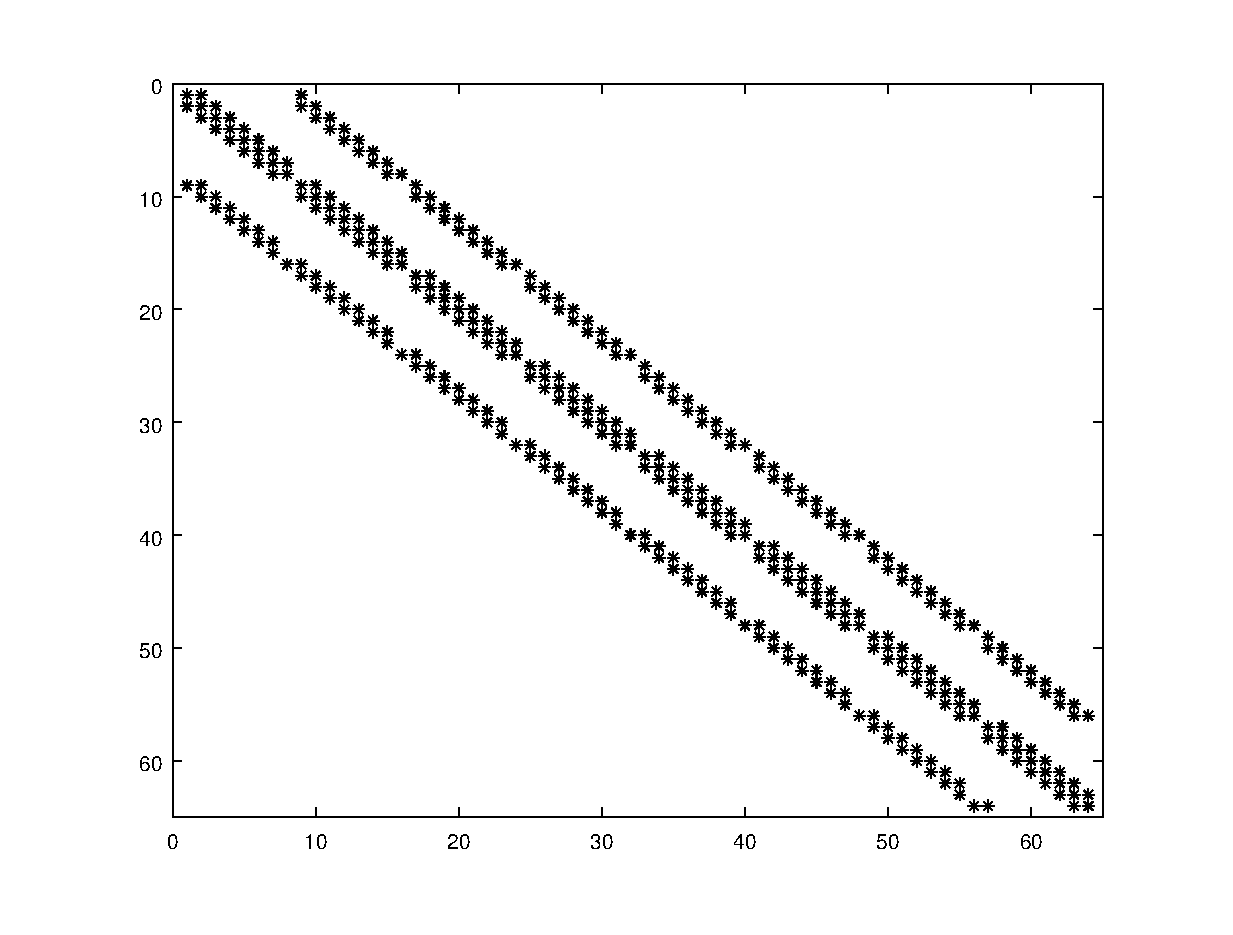
\includegraphics[width=0.38\textwidth , height=0.19\textheight]{pics/2d-7pt/2d_7pt_bw.eps}}
	\hspace{1em}
	\subfloat[Graph]{\label{fig:2d-7pt-c}\includegraphics[width=0.32\textwidth , height=0.18\textheight]{pics/2d-7pt/stencil_2d_7pt.pdf}}
	\caption{Basic structure of an artificially designed stencil (a) as well as corresponding sparsity pattern of its matrix discretization (b) and graph representation (c). A $8 \times 8$ lattice in two dimensions with Dirichlet boundary conditions are chosen. The stencil structure is designed for illustration purpose and does not represent any specific application scenario.}
	\label{fig:2d-7pt}
\end{figure}

\subsection*{Definitions}
The following basic definitions from graph theory are used in the following sections:
\begin{itemize}
	\item \textbf{Graph : } $G = (V,E)$ represents a graph where $V(G)$ belongs to set of vertices and $E(G)$ represents the edges in the graph. Note that we use $G$ for irreducible undirected graphs.
	\item \textbf{Neighborhood :} Neighborhood of vertex $u$ represented as $N(u)$ is defined as:
	\begin{equation*}
	  N(u) = \set{ v : uv \in E}.
	\end{equation*}
	\item \textbf{Subgraph :} In this paper a subgraph $H$ of graph $G$ specifically refers to the subgraph induced by vertices $V' \subseteq V(G)$ and is defined as
	\begin{equation*}
		H = (V', \set{ uv : uv \in E(G) \text{ and } u,v \in V'}).
	\end{equation*}
\end{itemize}

\subsection{Level Construction}\label{subsec:LEVEL_CONST}
The first step of \RACE is to determine different \levels in the graph followed by a related permutation of the graph data structure. This is equivalent to well-known bandwidth reduction algorithms such as ``(Reverse) \CMfull" or ``Breadth First Search" (\BFS) \cite{BFS} based approaches. Though the RCM method is implemented in \RACE, we use the  \BFS reordering in the following for better illustration purpose.
%\BFS can also be replaced with better bandwidth reduction algorithms like ``(Reverse) \CMfull".  
As a first step we choose a root vertex which is assigned to the first level ($L(0)$). All other levels ($L(i)$ for $i > 0$) are defined to  contain vertices that are in neighborhood of vertices in previous \level $L(i-1)$ but not in level $L(i-2)$ \cite{BFS_level_def} \ie
\begin{equation}\label{eq:level}
L(i) = 
\begin{cases}
	  u : u \in N(L(i-1)) \cap \overline{N(L(i-2))}  & \text{ if } i \neq 0, \\
	 root & otherwise.
\end{cases}   
\end{equation}

From \cref{eq:level} one finds that the $i$-th \level consist of all vertices that have a minimum distance of $i$ from the root node. See \Cref{alg:BFS} on how to determine minimum distance of each node from the root. The total number of levels obtained with this graph traversal is denoted as \totalLvl. \Cref{fig:2d_7pt_level_construction} shows the \totalLvl=14 \levels of an artificial stencil discretization, where the index of each vertex ($v$) refers to the vertex number and the superscript represents the \level number, \ie
\begin{equation}\label{eq:node_notation}
	v^i \implies v \in L(i).
\end{equation}
Note that this is substantially different to the \levels used in ``level-scheduling" \cite{saad} approach which applies a "Depth First Search".

\begin{figure}[tbhp]
	\centering
	\subfloat[Level construction]{\label{fig:2d_7pt_level_construction}\includegraphics[height=0.18\textheight,width=0.32\textwidth]{pics/level_construction/stencil_2d_7pt}}
	\hspace{1em}
	\subfloat[Permuted graph ($G'$)]{\label{fig:2d_7pt_perm}\includegraphics[height=0.18\textheight,width=0.32\textwidth]{pics/permutation/stencil_2d_7pt}}
	\hspace{1em}
	\subfloat[]{\label{fig:2d_7pt_levelPtr}\includegraphics[height=0.18\textheight,width=0.07\textwidth]{pics/permutation/levelPtr}}
	\caption{Levels of the original graph (a) and the permuted graph (b) for the \stex. The entries of  the \levelPtr associated with $G'$ are presented in (c).}
	\label{fig:2d-7pt_step_1_2}
\end{figure}


%\subsection{Permutation}\label{subsec:PERM}
After the \levels have been determined, the matrix is permuted in the order of its \levels, such that the vertices in $L(i)$ are stored consecutively and appear before that of $L(i+1)$. \Cref{fig:2d-7pt_step_1_2} displays the graph ($G' = P(G)$) of \stex after applying this permutation ($P$) and demonstrates the enhanced spatial locality of the vertices within an level (see \cref{fig:2d_7pt_perm}) as compared to the original (lexicographic) numbering (see \cref{fig:2d_7pt_level_construction}).  Until now the procedure is the same as \BFS (or \RCM). 

As \RACE uses information about the \levels for resolving dependencies in the coloring step, we store the entry point to each level in the permuted data structure (of $G'$) in an array $\levelPtr[0:$ \totalLvl$]$, i.e. \levels on $G'$ can be identified as:
\begin{equation*}
	L(i) = \set{ u : u \in [\levelPtr[i]:(\levelPtr[i+1]-1)] \text{ and } u \in V(G')} .
\end{equation*}

The entries of \levelPtr for \stex are shown in \cref{fig:2d_7pt_levelPtr}. 
%, and one could easily read from \levelPtr that vertices from $\levelPtr(4)=7$ to $\levelPtr(5)-1=10$ belongs to $L(4)$.
 
 \subsection{Distance-k coloring} \label{subsec:DK}
 The \levels generated above serve as the base for our \DK coloring procedure as they contain information about the neighborhood relation between the vertices of any two levels. Following the definition in~\cite{dist_k_def}, two vertices are called \DK neighbors if the shortest path connecting them consists of at most $k$ edges.
%In this section we introduce the idea of \DK neighbor and show how this idea can be used to color the matrix with the help of the level information that we already have in hand.
This implies $u$ is a \DK neighbor of $v$ (denoted as $u\xrightarrow{k}v$)  if
 \begin{equation}\label{eq:dk}
	  u\xrightarrow{k}v  \iff  v \in \set{ u \cup N(u) \cup N^2(u) \cup ... N^k(u) }.	 
 \end{equation}
 For undirected graphs as considered in this work  $u\xrightarrow{k}v$ also implies $v\xrightarrow{k}u$. Based on this definition we consider two vertices to be \DK independent if they are not \DK neighbors. Thus,  \levels $L(i)$ and $L(i+k+j)$  of the permuted graph $G'$ are \DK independent for all $j\geq1$ as shown in the following:
  \begin{corollary}\label{corollary_dk}
   $L(i)$ and $L(i\pm(k+j))$ are \DK independent $\forall j\geq1$. 
  \end{corollary}
  \begin{proof}
  	We prove by contradiction. Let there exist $u,v \in V(G')$ such that  $u \in L(i)$ and $v \in  L(i \pm (k+j)) \forall j\geq1$. Assume $u,v$ are \DK neighbors ($u\xrightarrow{k}v$). From \cref{eq:level}, \cref{eq:dk} and the fact $G'$ is undirected we get 
  	\begin{align*}
	  	u\xrightarrow{k}v \iff & v \in \set{L(i) \cup L(i \pm 1) \cup ... \cup L(i \pm k)} \\
	  	\implies & v \notin L(i \pm (k+j) \text{  } \forall j \geq 1
  	\end{align*}
  	which contradicts to $v \in L(i \pm (k+j) ) \forall j \geq 1$. This implies $u$ and $v$ are \DK independent.
  \end{proof}

\Cref{corollary_dk} implies that if there is a gap of \emph{\atleast} one \level between any two \levels ($L(i), L(i+2)$ for example) all the vertices between them are \DONE independent. Similarly if the gap consists of \emph{\atleast} two \levels between any two \levels ($L(i), L(i+3)$ for example) we have \DTWO independent levels.
  
 \begin{figure}[tbhp]
 	\centering
 	\subfloat[\DONE independent \levelGroups]{\label{fig:2d_7pt_d1}\includegraphics[height=0.2\textheight,width=0.4\textwidth]{pics/dk_coloring/stencil_2d_7pt_d1}}
 	\hspace{2.5em}
 	\subfloat[\DTWO independent \levelGroups]{\label{fig:2d_7pt_d2}\includegraphics[height=0.23\textheight,width=0.48\textwidth]{pics/dk_coloring/stencil_2d_7pt_d2_with_lg}}
 	\caption{Forming \DONE and \DTWO independent \levelGroups for the \stex.}
 	\label{fig:2d-7pt_d1_d2}
 \end{figure}
 
 % {\CA Maybe more explanation is required.} 
 The weak definition used in \cref{corollary_dk} offers many choices for forming \DK independent sets of vertices, which can then be executed in parallel. 
 In  \Cref{fig:2d_7pt_d1}  and \Cref{fig:2d_7pt_d2} we present one example for \DONE and \DTWO coloring of our \stex, respectively. The \DONE coloring uses a straight forward approach by assigning two colors to alternating levels, i.e. \levels of a color can be calculated concurrently. In case of \DTWO independency we refrain from using three colors but instead aggregate two adjacent \levels to form a \levelGroup (denoted by $T(i)$) and perform a \DONE coloring on top of those groups. This guarantees that vertices of two \levelGroups of the same color are \DTWO independent and can be executed in parallel. Here, the vertices in $T(0)$, $T(2)$, $T(4)$, $T(6)$ can be operated by four different threads in parallel, i.e. one thread per \levelGroup.  After synchronisation the remaining four blue \levelGroups can also be executed in parallel. Note, that within a single \levelGroup all verticies are computed in their original order enabling high spatial locality for accessing them. This idea can be generalized such that for \DK coloring, \levelGroups containing at least $k$ adjacent \levels need to be formed and \DONE coloring of the \levelGroups is done on top. Then, all \levelGroups within a color can be executed in parallel. This simple approach allows to generate workload for $\frac{\totalLvlMATH}{2 k}$ threads if \DK coloring is requested.
 
However, choosing the same number of \levels for each \levelGroup may lead to severe load imbalances as can be seen in \cref{fig:2d-7pt_d1_d2}. In particular the use of bandwidth reduction schemes such as BFS or RCM will further worsen that problem due to the shape like matrix structures generated leading to low workload for matrix rows at the top and bottom of the matrix. Compare \eg $T(1)$ and $T(7)$ with  $T(3)$ and $T(4)$ in \cref{fig:2d-7pt_d1_d2}.
 %coloring by aggregating consecutive levels into \levelGroups (denoted by $T(i)$). In  \Cref{fig:2d_7pt_d1}  and \Cref{fig:2d_7pt_d2} we present one example for \DONE and \DTWO coloring of our \stex, respectively. The \DONE coloring uses straight forward approach by assigning two colors to alternating levels, i.e. \levelGroup and \level is equivalent here. For and applying a \DONE coloring on top of those groups as shown for \DTWO coloring in \cref{fig:2d_7pt_d2}.  In this context \Cref{fig:2d-7pt_d1_d2} contains two potential colorings for \DONE independent \levels as \DTWO coloring also solves \DONE dependencies.  One could also group some more of nearby \levels together to form a \levelGroup, and make this \DONE or \DTWO independent of other \levelGroups. The $i$-th \levelGroup would be denoted by $T(i)$. Difference between \level and  \levelGroup can be seen in \cref{fig:2d_7pt_d2}, for \cref{fig:2d_7pt_d1} \levelGroup and \level coincides. In principle one could compute on all independent \levelGroups in parallel, but sequentially within a \levelGroup, \ie for example in \cref{fig:2d_7pt_d2} $T(0)$, $T(2)$, $T(4)$, $T(6)$ can be operated by four different threads in parallel and in the next sweep rest \levelGroups. For the configurations seen in \cref{fig:2d-7pt_d1_d2} then we have $\frac{\totalLvlMATH}{2}$ and $\frac{\totalLvlMATH}{4}$ parallelism for \DONE and \DTWO kernels respectively.
  %However the problem with the configurations like the one seen in \cref{fig:2d-7pt_d1_d2} {\CA is that there, check Holger's comment} is load imbalances between threads because the number of rows (\nrows) per \levelGroup is not distributed evenly. As seen here in the case of \stex the threads working on extreme ends of graph (\eg $T(1), T(7)$) have a small amount of work compared to the threads working on middle (\eg $T(3), T(4)$). 
  
  \subsection{Load balancing}\label{subsec:LB}
  Depending on the matrix each \levelGroup contains different number of rows, that leads to load imbalances as {\CA seen above} in \cref{subsec:DK}. \Inorder to avoid this problem we employ a load balancing scheme. At this step  we plug in details from the hardware side  namely the total parallelism required by the hardware. The idea is to exploit only the required parallelism while at the same time maintain \DK constraint seen in \cref{corollary_dk}. To balance the load more nearby \levels would be added to a \levelGroup ($T(x)$) which has less number of rows ($\nrowsMath(T(x))$) and at \levelGroup where we have considerably big \levels only sufficient amount of \levels to maintain \DK constraint would be assigned. Assigning nearby levels instead of others further helps in preserving data locality. 
  
  An algorithm for load balancing can be found in \cref{alg:LB}. The aim of the algorithm is to reduce combined variance of number of rows ($\nrowsMath(T(i))$) in each \levelGroup $T(i)$. It does this by calculating mean and variance of $T\_size$ in each parallel sweeps, where $T\_size(i)$ is $\nrowsMath(T(i))$(number of rows in $T(i)$). For example in \cref{fig:2d_7pt_d2} we need to calculate mean of $T\_size$ of all \levelGroups in red sweep and blue sweep separately. The combined variance is then found by summing up the variances in each parallel sweep. \Inorder to reduce this combined variance we select the \levelGroup that has biggest absolute deviation from mean and try to add/remove levels to/from this \levelGroup from/to a \levelGroup that has biggest/least signed deviation. While removing \levels from a \levelGroup one has to take care that the \DK coloring is not violated, for example in case of \DTWO and two sweep scheme as seen in \cref{fig:2d_7pt_d2} we need to ensure at least two levels remain in a \levelGroup. To aid this shifting of \levels we use a pointer denoted as $T\_ptr$. $T\_ptr$ points to the beginning of each \levelGroup, therefore shifting them changes the size of \levelGroups. Doing this process in an iterative way finally we end up in a state with lowest combined variance at which no further moves are possible either due to violation of \DK dependency or due to increase in combined variance. \Cref{fig:lb_alg} shows step by step procedure involved in load balancing and \cref{fig:2d_7pt_lb} shows \levelGroups after load balancing applied on \stex of size $16 \times 16.$

  One could also do this entire load balancing based on number of non-zeros (\nnz) rather than \nrows, in this case $T\_size(i)=\nnzMath(T(i))$ (non-zeros in $T(i)$).
  
   \begin{figure}[tbhp]
   	\centering
   	\includegraphics[height=0.22\textheight,width=\textwidth]{pics/load_balancing/lb_alg/lb_all}
   	\caption{Steps in load balancing (clockwise starting from top-left)}
   	\label{fig:lb_alg}
   \end{figure}
   
    
    \begin{figure}
      \begin{minipage}[c]{0.63\textwidth}
      	\includegraphics[height=0.26\textheight,width=0.9\textwidth]{pics/load_balancing/2d-7pt/stencil_2d_7pt}
      \end{minipage}\hfill
      \begin{minipage}[c]{0.34\textwidth}
      	\caption{After load balancing for five threads and \DTWO dependency on \stex, domain size $16 \times 16$. Note that \levelGroups at extreme end have more \levels due to less \nrows in each \level, while \levelGroups in middle having bigger \levels maintain two levels to preserve \DTWO constraint.
      	} \label{fig:2d_7pt_lb}
      \end{minipage}
     \end{figure}
     

	\subsection{Recursion}\label{subsec:REC}
	As seen above in \cref{subsec:DK} maximum amount of parallelism by the above approach depends on total number of levels (\totalLvl), also for most of the graphs as we approach the limit of parallelism there is not much room for load balancing, leading to imbalances. Depending on matrix and hardware underneath this might lead to inefficient utilization of resources. \Inorder to avoid this problem we use the concept of recursion and exploit further parallelism if required by the hardware. Idea here is to intelligently select sub-graph(s) of the entire matrix and apply all the three steps recursively on this \subgraph. In the following we will show this concept in the context of \DONE and  later we will extent it to \DK dependencies. In order to explain the basic concepts easily and include all the corner cases we demonstrate the procedure on a simple graph as shown in \cref{fig:rec_d1_s1_a}, later we will show the results of applying recursion on \stex. Further we will discuss on the method employed to select proper sub-graph and to have a globally balanced load.
	
	\subsubsection{Distance-$1$}
	\LevelGroups which we constructed till now belong to first stage of recursion ($s=0$). Stage number of recursion is denoted using subscript, \ie for example $L_s(i)$ denotes \level $i$ of stage $s$. Contrary to methods like \MCfull we didn't require each nodes in a color to be \DONE independent of each other, rather we had a weak constraint as prescribed by \cref{corollary_dk}. Due to this there can exist more parallelism within a \levelGroup. For example in \cref{fig:rec_d1_s1} we see that within third \levelGroup of first stage (T$_0$(2)) vertices $4 \not\xrightarrow{1} 5$ ($4$  \DONE independent to $5$), $4 \not\xrightarrow{1} 6$, $4 \not\xrightarrow{1} 7$ and $5 \not\xrightarrow{1} 7$, implying each of these pairs can be computed in parallel without any \DONE conflicts. This parallelism couldn't be exploited in first stage ($s=0$)  since vertices in $L_0(i)$ (here $i=2$) were connected to preceding \level $L_1(i-1)$ although some of them were not \DONE dependent within $L_0(i)$. \Inorder to exploit this parallelism we use the concept of recursion.
	
     \begin{figure}[thbp]
     	\centering
     	\subfloat[Example graph]{\label{fig:rec_d1_s1_a}\includegraphics[width=0.26\textwidth, height=0.14\textheight]{pics/recursion/d1/rec_graph_s1/recursion_graph_1}}
     	\hspace{1.5em}
     	\subfloat[Stage 1 levels in graph]{\label{fig:rec_d1_s1_b}\includegraphics[width=0.26\textwidth, height=0.14\textheight]{pics/recursion/d1/rec_graph_s1/recursion_graph_2}}
     	\hspace{1.5em}
     	\subfloat[\DONE coloring]{\label{fig:rec_d1_s1_c}\includegraphics[width=0.26\textwidth, height=0.14\textheight]{pics/recursion/d1/rec_graph_s1/recursion_graph_3}}
        \caption{Shows potential for more parallelism. $T_0(1),T_0(2)$ and $T_0(3)$ has more parallelism. Note that the graph shown here is not related to the previous \stex.}
     	\label{fig:rec_d1_s1}
     \end{figure}
     
     Recursion begins by selection of a \subgraph of the matrix. A typical choice is a \subgraph induced by vertices in a \levelGroup of previous stage, more on the selection of \subgraph will be seen later in \cref{subsec:subgraph_selection}. For example let's choose \subgraph induced by $T_0(2)$ for recursion. The chosen \subgraph can be isolated from rest of the graph since  \DONE coloring step in stage 0 has already made \levelGroups in a sweep independent of each other. Now we just need to repeat all the three steps explained previously (\cref{subsec:LEVEL_CONST} - \cref{subsec:LB}) to exploit parallelism within this \subgraph.
   
     \begin{figure}[thbp]
     	\centering
     	\subfloat[]{\label{fig:rec_d1_s2_a}\includegraphics[width=0.26\textwidth, height=0.14\textheight]{pics/recursion/d1/rec_graph_s2/recursion_graph_stage2_1}}
     	\hspace{2.25em}
     	\subfloat[]{\label{fig:rec_d1_s2_b}\includegraphics[width=0.08\textwidth, height=0.14\textheight]{pics/recursion/d1/rec_graph_s2/recursion_graph_stage2_2}}
     	\hspace{1.75em}
     	\subfloat[]{\label{fig:rec_d1_s2_c}\includegraphics[width=0.07\textwidth, height=0.14\textheight]{pics/recursion/d1/rec_graph_s2/recursion_graph_stage2_3}}
     	\hspace{1.75em}
     	\subfloat[]{\label{fig:rec_d1_s2_d}\includegraphics[width=0.07\textwidth, height=0.14\textheight]{pics/recursion/d1/rec_graph_s2/recursion_graph_stage2_4}}
	     \hspace{1.75em}
	     \subfloat[]{\label{fig:rec_d1_s2_e}\includegraphics[width=0.07\textwidth, height=0.14\textheight]{pics/recursion/d1/rec_graph_s2/recursion_graph_stage2_5}}
     	\caption{Shows recursion being applied to $T_0(2)$. \Cref{fig:rec_d1_s2_b} shows the selected \subgraph, \cref{fig:rec_d1_s2_c} shows level construction step on the \subgraph, \cref{fig:rec_d1_s2_d,fig:rec_d1_s2_e} shows two possibility of \DONE coloring of the \subgraph}
     	
     	\label{fig:rec_d1_s2}
     \end{figure}
     
     \Cref{fig:rec_d1_s2} shows an illustration of applying second stage ($s=1$) of recursion on $T_0(2)$. To incorporate the information of levels in different stages of recursion onto the vertices we extent the definition in \cref{eq:node_notation} to the following:
	 \begin{equation}
	    v^{i,j,k...} \implies v \in \set{L_1(i) \cap L_2(j) \cap L_3(k) \cap ...} 
	 \end{equation}
	 
     In this case at the end of recursion (\cf \cref{fig:rec_d1_s2_d}, \cref{fig:rec_d1_s2_e}) on $T_0(2)$ we obtain parallelism for two more threads. Note that the \subgraphs might have multiple islands (group of vertices in a graph that are not connected to rest of the graph). For example vertex 3 in \cref{fig:rec_d1_s2_b} is an island in the considered \subgraph, similarly vertices 4,5,6 combine to form an island. Since an island is totally disconnected from the rest of the graph it can be executed in parallel to rest of the graph. To take advantage of this the starting node in next island is assigned with an increment of two levels, as seen in \cref{fig:rec_d1_s2_c}. Due to this there exists multiple valid \DONE configuration (\cf \cref{fig:rec_d1_s2_d,fig:rec_d1_s2_e}) and the selection of the optimal one will be done in the final load balancing step of a particular stage as described in \cref{subsec:LB}.    
     
     With this recursive process we were able to find independent \levelGroups ($T_{s+1}$) within \levelGroup of previous stage ($T_s$) and therefore the thread which works on $T_s$ has to spawn threads to parallelize within $T_{s+1}$.
     
	\subsubsection{Distance-$k$}
	For \DK the same procedure as \DONE applies, except with a slight difference in selecting the \subgraph. In \DONE we considered \subgraphs induced by \levelGroups, but for \DK coloring this is not sufficient. As seen in \cref{fig:rec_d2_wrong} for \DTWO coloring the selection of $T_0(1)$ as \subgraph did not guarantee \DTWO independency within \levelGroup $T_1$ of the \subgraph, for \eg $T_1(0)$ and $T_1(2)$ are not \DTWO independent (\cf \cref{fig:rec_d2_wrong_d}). This is due to the fact that for $k>1$ dependencies two vertices $a,b$ within a \subgraph might be connected to a common vertex ($c$) outside the \subgraph leading to a \DK dependency between $a$ and $b$. In \cref{fig:rec_d2_wrong} we see 	$3 \xrightarrow{1} 1 \text{ \& } 6 \xrightarrow{1} 1 	\implies 3 \xrightarrow{2} 6$, but since vertex $2$ was not in the \subgraph considered we missed this dependency. 

	
     \begin{figure}[thbp]
     	\centering
     	\subfloat[]{\label{fig:rec_d2_wrong_a}\includegraphics[width=0.23\textwidth, height=0.13\textheight]{pics/recursion/d2/wrong/recursion_graph_wrong_1}}
     	\hspace{0.6em}
     	\subfloat[]{\label{fig:rec_d2_wrong_b}\includegraphics[width=0.23\textwidth, height=0.07\textheight]{pics/recursion/d2/wrong/recursion_graph_wrong_2}}
     	\hspace{0.6em}
     	\subfloat[]{\label{fig:rec_d2_wrong_c}\includegraphics[width=0.23\textwidth, height=0.07\textheight]{pics/recursion/d2/wrong/recursion_graph_wrong_3}}
     	\hspace{0.6em}
     	\subfloat[]{\label{fig:rec_d2_wrong_d}\includegraphics[width=0.23\textwidth, height=0.13\textheight]{pics/recursion/d2/wrong/recursion_graph_wrong_4}}
     	\caption{\Cref{fig:rec_d2_wrong_a,fig:rec_d2_wrong_b} shows \levelGroup induced \subgraph selected for recursion in case of \DTWO. But applying the three steps to this selected \subgraph does not guarantee a \DTWO independency between \levelGroup of same sweep (color) as seen in \cref{fig:rec_d2_wrong_d}}
     	\label{fig:rec_d2_wrong}
     \end{figure}
   
   \Inorder to resolve such dependency we have to consider an extra $(k-1)^{th}$ interface level(s) of the selected \subgraph for the level construction step. The $k^{th}$ interface level(s) of subgraph $T_s(j)$, denoted as $I^k(T_s(j))$, is defined as follows:
   \begin{equation*}
	   I^k(T_s(j)) = \set{u : u \xrightarrow{k} v \text{  } \forall v \in T_s(j) \text { and } u \notin T_s(j)}
   \end{equation*}
   For \DTWO this would mean we have to include $1^{st}$ interface level, the new selection is illustrated in \cref{fig:rec_d2_correct}. If we then do all the three steps with the newly created \subgraph, the final result will preserve \DTWO coloring (see \cref{fig:rec_d2_correct_c}). In the example it can be observed vertices $3$ and $6$ which previously had same color now get assigned to different colors (see \cref{fig:rec_d2_correct_d}). Note that the interface levels have to be considered only in the first step namely level construction in the rest of the steps we just need to consider target \subgraphs induced by \levelGroups \ie in \cref{fig:rec_d2_correct} the \subgraph induced by $T_0(1)$. 
   
     
     \begin{figure}[thbp]
     	\centering
     	\subfloat[]{\label{fig:rec_d2_correct_a}\includegraphics[width=0.22\textwidth, height=0.13\textheight]{pics/recursion/d2/correct/recursion_graph_correct_1}}
     	\hspace{0.6em}
     	\subfloat[]{\label{fig:rec_d2_correct_b}\includegraphics[width=0.22\textwidth, height=0.105\textheight]{pics/recursion/d2/correct/recursion_graph_correct_2}}
     	\hspace{0.6em}
     	\subfloat[]{\label{fig:rec_d2_correct_c}\includegraphics[width=0.22\textwidth, height=0.105\textheight]{pics/recursion/d2/correct/recursion_graph_correct_3}}
     	\hspace{0.6em}
     	\subfloat[]{\label{fig:rec_d2_correct_d}\includegraphics[width=0.22\textwidth, height=0.105\textheight]{pics/recursion/d2/correct/recursion_graph_correct_4}}
     	\hspace{0.6em}
     	\caption{Correct procedure of selecting \subgraph for \DTWO coloring. The \levelGroup $T_0(1)$ and it's $1^{st}$ interface level is chosen as the \subgraph as shown in \cref{fig:rec_d2_correct_a,fig:rec_d2_correct_b}. Level construction step is then applied to this \subgraph as seen in \cref{fig:rec_d2_correct_c}. Rest of the steps like permutation and \DK coloring is applied only to the \subgraph  chosen for recursion (here $T_0(1)$). Finally as seen in \cref{fig:rec_d2_correct_d} we get three \levelGroups at the end of recursion on $T_0(1)$.}
     	\label{fig:rec_d2_correct}
     \end{figure}
     

       \begin{figure}[H]
       	\begin{minipage}[c]{0.6\textwidth}
       		\includegraphics[height=0.3\textheight,width=0.89\textwidth]{pics/recursion/2d-7pt_example/2d-7pt/stencil_2d_7pt}
       	\end{minipage}\hfill
       	\begin{minipage}[c]{0.4\textwidth}
       	%	{\tt for parallel all \textcolor{red}{red}\\
       	%		\hspace*{1em} for parallel all \textcolor{amber}{orange}\\
       	%		\hspace*{1em} for parallel all \textcolor{magenta}{pink}\\
       	%	}
       	%	{\tt for parallel all \textcolor{blue}{blue}\\
       	%		\hspace*{1em} for parallel all \textcolor{carmine}{brown}\\
       	%		\hspace*{1em} for parallel all \textcolor{cyan}{cyan}\\
       	%	}
	       	\begin{tabular}{l|l}
	    %   		\toprule
	       		{No recursion} & {$s=1$ recursion}\\
	       		\midrule
	       	   \multirow{2}{*}{\textcolor{red}{red}} & {\textcolor{amber}{orange}}\\
	       	   \cmidrule(lr){2-2}
	       		& {\textcolor{magenta}{pink}}\\
	       		\midrule
	       	   \multirow{2}{*}{\textcolor{blue}{blue}} & {\textcolor{carmine}{brown}}\\
	       	   \cmidrule(lr){2-2}
	       	   & {\textcolor{cyan}{cyan}}\\
	       	   \bottomrule
	       	\end{tabular}
       		\caption{Recursion applied to \stex for eight threads. Here recursion is applied on \levelGroups $T_1(4-7)$, to get two threads each. The execution order of different \levelGroup is specified in the illustration towards right. Vertical line distinguishes between \levelGroups with and without recursion and each horizontal line denotes the required synchronization. Note the requirement of nested parallelism.}
       		\label{fig:rec_2d-7pt_graph}
       	\end{minipage}
       \end{figure}
     
     \Cref{fig:rec_2d-7pt_graph} (left) shows \DTWO coloring of \stex  for eight threads. Here we see recursion is applied to \levelGroups $T_0(4),T_0(5),T_0(6)$ and $T_0(7)$. In this case each of the \levelGroups where recursion is applied spawns parallelism for two threads. The selection of \levelGroups to refine and number of threads needed from each recursion are determined using a global load balancing technique as will be explained in \cref{subsec:subgraph_selection}.
     
      \Cref{fig:rec_2d-7pt_graph} (right) shows the execution order of different \levelGroups. Note the usage of nested parallelism, \ie for example thread responsible for $T_0(4)$ spawns two child threads to execute $T_1(0) \subset T_0(4)$ and $T_1(2) \subset T_0(4)$ in one parallel sweep, and $T_1(1) \subset T_0(4)$ and $T_1(3) \subset T_0(4)$ in next parallel sweep. At the end of each sweep there is synchronization between threads assigned to \levelGroup of similar color. Since each of the leaf need to synchronize only with it's siblings (leaves of same parent)  we use simple point to point synchronization scheme. 
          
       
	\subsubsection{Internal representation of recursively generated \boldmath{\levelGroups}} \label{subsec:level_tree}
	The recursive nature of our procedure allows to exploit more parallelism. However this introduces more complexity and one has to additionally respect the dependencies between stages and still observe the dependencies within one stage. The best idea is to have a data structure similar to the recursion, therefore we extent the \levelPtr data structure to a hierarchical tree data structure to store these informations. This data structure is called a \levelTree. The root of \levelTree contains information of entire domain, first child leaves of this root \ie leaves with depth 1 stores information about \levelGroups in first stage ($T_0(..)$), leaves with depth 2 stores information about \levelGroups in second stage ($T_1$) and so on. 
	
	 \begin{figure}[thbp]
		 \includegraphics[width=\textwidth, height=0.2\textheight]{pics/recursion/2d-7pt_example/tree/tree}
	 	\caption{\levelTree corresponding to \stex for domain size $16 \times 16$, and 8 threads. The range (square brackets) specified in each leaves represent the vertices belonging to each \levelGroup, the \nrowsEff (see \cref{Sec:param_study}) is represented within angle brackets, and the id refers to the thread id assigned to each \levelGroups assuming compact pinning .}
	 	\label{fig:rec_2d-7pt_tree}
	 \end{figure}

 
 \Cref{fig:rec_2d-7pt_tree} shows a \levelTree corresponding for \stex  with 8 threads as seen in \cref{fig:rec_2d-7pt_graph}. The leaves in the tree correspond to different \levelGroups and store various informations like the range of vertices or nodes that belong to this \levelGroup, the effective number of rows (\nrowsEff) that describes the quality of the method (which we will see later in \cref{Sec:param_study}), and other informations like threads assigned to specific \levelGroups.  Threads are assigned to each \levelGroup depending on the pinning strategy used. For example in \emph{fill} type pinning strategy one would pin thread 0 to $T_0(0)$ and $T_0(1)$, thread 1 to $T_0(2)$ and $T_0(3)$, thread 2 to $T_1(0)  \subset T_0(4)$, $T_1(1) \subset T_0(4)$, $T_1(0)  \subset T_0(5)$ and $T_1(1) \subset T_0(5)$, and so on as seen in \cref{fig:rec_2d-7pt_tree}. 
 
 Note that the \levelTree has a data structure that represents the nested parallelism being used as seen in \cref{fig:rec_2d-7pt_graph} (right). Therefore threads are spawned based on this \levelTree allowing for easy implementation of point to point synchronizations.

\subsubsection{Sub-graph selection and global load balancing} \label{subsec:subgraph_selection}
Parallelism required for hardware underneath can be obtained either by expanding the \levelTree horizontally \ie increasing \levelGroups within a stage or by expanding \levelTree vertically with the help of recursion. But as we have seen before in \cref{subsec:DK} the horizontal parallelism is limited and after a certain extent this would lead to load balancing. Similarly excessive usage of recursion is also not a good idea since data locality worsens due to local permutations within \subgraph. Therefore it is vital to find a proper balance and choose proper configuration. Furthermore just doing load balancing within a single stage is not the best, for example if we had equally balanced within stage 1 in \cref{fig:rec_2d-7pt_tree}, we would receive no benefit from recursion. Therefore a global load balancing becomes inevitable.

\Inorder to select proper \subgraph and do global load balancing we employ a simple algorithm to find proper weights for each \levelGroup ($T_s(i)$) in a particular stage, then depending on this weights, denoted as $w(T_s(i))$, we do load balancing with weights in the particular stage (as seen in \cref{alg:LB}, except weightage is given to \levelGroups). Finally if $w(T_s(i)) > 1$ we use recursion to achieve $w(T_s(i))$ parallel work in the next stage of $T_s(i)$. The basic structure of the algorithm employed to find weights for the first stage is as follows:
\begin{enumerate}
	\item Find weights, $w(L_0(i))$ for each level in the current stage ($s$) by
		\begin{align*}
			w(L_0(i)) &= (\levelPtr_0[i+1] - \levelPtr_0[i])*\frac{\nthreadsMath}{\nrowsMath^{total}}\\
			\nthreadsMath &: \text{total parallelism required by hardware}\\
			\nrowsMath^{total} &: \text{number of vertices in graph}
		\end{align*}
	
	\item Starting from $w(L_0(0))$ sum up weights till they form a number ($a$) close to whole number ($b$). The closeness can be controlled by an efficiency parameter for stage $s$, $\epsilon_s$ is defined as:
	\begin{equation} \label{eq:epsilon}
		\epsilon_s =  1 - abs(a-b);
	\end{equation}
	All the \levels that are involved in the sum belongs to \levelGroups  operated by first thread in the current stage. The obtained number $b$ is chosen as weight for these \levelGroups \ie $w(T_0(0))=w(T_0(1))=b$. A local search is then done by increasing \levels in this \levelGroups to see if there is a better choice ($a$ close to $b$) with weight $b$, finally \levelGroups are formed with the best choice.  The weight for next \levelGroups are found by resetting the sum counter to zero and repeating the  procedure with \levels just after the current \levelGroups.
\end{enumerate}
For other recursive stage ($s\geq1$) same procedure can be applied to find weights $w(T_s(i))$, except that now $\nthreadsMath$ and $\nrowsMath^{total}$ has to be substituted with the threads required and vertices in the \subgraph considered.

\section{Parameter study}
\label{Sec:param_study}
% SIAM Shared Information Template
% This is information that is shared between the main document and any
% supplement. If no supplement is required, then this information can
% be included directly in the main document.

%In this section we study the impact of parameter $\epsilon_s$ and hardware parallelism on the quality of  \acrshort{RACE} method. \Inorder to do this we first quantify the quality of the method and finally we  use this quantity to do a parameter study. The study gives insights into tuning of parameter $\epsilon_s$ based on the given matrix and required parallelism.


The \acrshort{RACE} method has a set of input
parameters $\{\epsilon_s; s=0,1,\ldots\}$ which control the
assignment of threads to adjacent level groups.
%For that reason a good choice is to have values close to $1$ for the initial stages and have a more relaxed constraint on the lower levels. 
To determine useful settings, we analyze the interaction
between these input parameters, the number of threads used, and the
parallel efficiency of the generated workload distribution.

As the internal tree structure contains all information about the
final workload distribution, we can use it to identify the critical
path in terms of workload and thus the parallel
efficiency. To this end we introduce the \effRow for every node
(or \levelGroup) $\acrshort{nrowsEff}(T_s(i))$, which is a measure for
the absolute runtime to calculate the
corresponding \levelGroup. For \levelGroups that are not further
refined (leaf nodes) this value is their actual workload, \ie the
number of rows assigned to them ($\acrshort{nrowsEff}(T_0(0)) = 15$
in \Cref{fig:rec_2d-7pt_tree}). For an inner node, the \effRow is the
sum of the maximum workload (\ie the maximum \effRow value) across each of
the two colors of its child nodes:
\begin{align*}
\acrshort{nrowsEff}(T_s(i)) &= \max\left(\acrshort{nrowsEff}(T_{s+1}(j) \subseteq T_s(i))\right) + \max\left(\acrshort{nrowsEff}(T_{s+1}(j+1) \subseteq T_s(i))\right)\\
 & \text{for } j=0,2,\ldots
\end{align*}
Such a definition is based on the idea that nodes at a given stage $s$
have to synchronize with each other and have to wait for their
siblings with the largest workload in each sweep (color). Propagating
this information upwards on the tree until we reach the root node
constructs the critical path in terms of longest runtime taking into
account single thread workloads, dependencies, and
synchronizations. Thus, the final value in the root node
$\acrshort{nrowsEff}(T_{-1}(0))$ can be considered as the effective
maximum workload of a single thread. Dividing the globally optimal
workload per thread,
${\acrshort{nrows}^\mathrm{total}}/{\acrshort{nthreads}}$, by
this number gives the parallel efficiency ($\eta$) of our workload
distribution:
\begin{align*}
	\eta &= \frac{ \acrshort{nrows}^\mathrm{total}} {\acrshort{nrowsEff}(T_{-1}(0)) \times \acrshort{nthreads}}. 
\end{align*}
For the tree presented in \Cref{fig:rec_2d-7pt_tree}, the parallel
efficiency is limited to $\eta=\frac{256}{44 \times 8 } = 0.73$ on
eight threads, \ie the maximum parallel speedup is $5.8$.

\subsection{Parameter analysis and selection}
\label{subsec:param_analysis}
The parallel efficiency \acrshort{eta} as defined above can be calculated for
any given matrix, number of threads $\acrshort{nthreads}$, and choice of
$\{\epsilon_s; s=0,1,\ldots\}$; it reflects the quality of parallelism generated
by \acrshort{RACE} for the problem at hand.  This way we can understand the
interaction between these parameters and identify useful choices for
the $\epsilon_s$. Of course, running a specific kernel such
as \acrshort{SymmSpMV} on actual hardware will add further hardware and software
constraints such as attainable memory bandwidth or cost of synchronization.

As a first step we can limit the parameter space by simple corner case
analysis. Setting all parameters close to one requests high-quality load
balancing but may prevent our balancing scheme from terminating. In the extreme
case of $\{\epsilon_s=1; s=0,1,\ldots\}$ the scheme may generate only
two \levelGroups (one of each color) in each recursion, assign all threads to
them, and may further attempt to refine them in the same way.  The lowest
possible value of $\epsilon_s$ is the maximum deviation of a real number from
its nearest integer, which is $0.5$. A range of [$0.5$,$0.9$] for the
$\epsilon_s$ is therefore used in the following. For \rDel{a basic analysis}
\rAdd{an initial discussion} we have
selected the \emph{inline\_1} matrix (see \Cref{tab:test_mtx}) as it has a
rather small amount of parallelism and allows us to cover basic
scenarios. In \Cref{fig:inline_param_study} we demonstrate the impact of
different choices for $\epsilon_0$ and $\epsilon_1$ on the parallel efficiency
for thread counts up to 100, which is a useful limit for modern CPU-based
compute nodes.
%
\begin{figure}[t]
	\centering
	\subfloat[$\eta$ versus \acrshort{nthreads} for \emph{inline\_1} matrix, $\epsilon_1 = 0.5$ ]{\label{fig:inline-a}\includegraphics[width=0.45\textwidth , height=0.2\textheight]{pics/param_study/threads_vs_eff}}
	\hspace{1.5em}
	\subfloat[\acrshort{nthreads}=25]{\label{fig:inline-b}\includegraphics[width=0.45\textwidth , height=0.2\textheight]{pics/param_study/scaling_eps_1_25_threads}}
	
	\subfloat[\acrshort{nthreads}=45 ]{\label{fig:inline-c}\includegraphics[width=0.45\textwidth , height=0.2\textheight]{pics/param_study/scaling_eps_1_45_threads}}
	\hspace{1.5em}
	\subfloat[\acrshort{nthreads}=100 ]{\label{fig:inline-d}\includegraphics[width=0.45\textwidth , height=0.2\textheight]{pics/param_study/scaling_eps_1_100_threads}}
	\caption{Parameter study on the \emph{inline\_1} matrix. In \Cref{fig:inline-b,fig:inline-c,fig:inline-d} each of the lines in the plot are iso-$\epsilon_1$ and impact of $\eta$ with respect to $\epsilon_0$ is shown. $\epsilon_s$ for $s>1$ is fixed to $0.5$.}
	\label{fig:inline_param_study}
\end{figure}
%
For $s > 1$ we always set the minimum value of $\epsilon_s=0.5$. The limited
parallelism can be clearly observed in \Cref{fig:inline-a}, with efficiency
steadily decreasing with increasing thread count. At
$\epsilon_1=0.5$ there is only a minor impact of the parameter
$\epsilon_0$. In \Cref{fig:inline-b,fig:inline-c,fig:inline-d} the interplay
between these two parameters is analyzed at different thread counts in more
detail. We find that up to intermediate parallelism ($\acrshort{nthreads}=50$)
the exact choice has only a minor impact on the parallel efficiency (see $y$-axis
scaling). For larger parallelism the interplay becomes more intricate,
where too large values of $\epsilon_{0,1}$ may lead to stronger imbalance. Based
on this evaluation, we choose $\epsilon_{0,1}=0.8$ and $\epsilon_s=0.5$ for $s>1$
for all subsequent performance measurements. The quality of this choice in terms of
parallel efficiency for all matrices is presented
in \Cref{fig:param_all_mtx_stat}. Here we plot the $\eta$ value for all the
matrices over a large thread count. We find that our parameter setting achieves
parallel efficiencies \rDel{of 80\% or higher for a substantial fraction of the
matrices up to intermediate thread counts.}
\rAdd{of 75\% or higher for 75\% of the matrices up to an intermediate thread count of 40. }
   \begin{figure}[t]
   	\centering
   	\includegraphics[width=0.9\textwidth]{pics/param_study/scatter_plot}
   	\caption{Parallel efficiency $\eta$ versus \acrshort{nthreads} for all test matrices with $\epsilon_{0,1} = 0.8$ and $\epsilon_{s>1} = 0.5$.}
  	\label{fig:param_all_mtx_stat}
   \end{figure}
Representing the upper (lower) values in \Cref{fig:param_all_mtx_stat} is the
best (worst) case matrix \emph{Graphene-4096} (\emph{crankseg\_1}), exhibiting
almost perfect (very low) parallel efficiency at intermediate to high thread
counts.

Finally, we evaluate the scalability of RACE using these two corner cases and
the \emph{inline\_1} matrix as well as the \emph{parabolic\_fem} matrix, which
is small enough to fit into the cache.  In \Cref{fig:corner_cases_param} we
mimic scaling tests on one Skylake processor with up to 20 cores (\ie
threads) and plot the parallel efficiency $\eta$ as well as the maximum number
of threads which can be ``perfectly'' used \acrshort{threadEff} (\ie
$\acrshort{threadEff} = \eta\times\acrshort{nthreads}$).  The unfavorable structure
of the \emph{crankseg\_1} matrix puts strict limits on parallelism even for low
thread counts.  The combination of small matrix size with a rather dense
population (see \Cref{table:bench_matrices}) leads to large inner levels when
constructing the graph, triggering strong load imbalance if using more than six
threads. A search for better $\epsilon_s$ slightly changes the characteristic
scaling but not the maximum parallelism that can be extracted. For
the \emph{inline\_1} matrix we find a weak but steady decrease of the parallel
efficiency, which is in good agreement with the discussion
of \Cref{fig:inline_param_study}. The other two matrices scale very well in the
range of thread counts considered.


The corresponding performance measurements for the \acrshort{SymmSpMV} kernel
(see \Cref{sect:SymmSpmv}) on a single \SKX processor chip with 20 cores are
shown in \Cref{fig:corner_cases_scaling}.\footnote{For the benchmarking setup
see \Cref{Sec:expt}.}
%A strong relationship between the theoretical  (\Cref{fig:corner_cases_param}) and  experimental (\Cref{fig:corner_cases_scaling}) scaling graph can be clearly observed. 
For the \emph{crankseg\_1} matrix (see \Cref{fig:crankseg_scaling}) we recover
the limited scaling due to load imbalance as theoretically predicted. A
performance maximum is at nine cores, where the maximum \acrshort{SpMV}
performance can be slightly exceeded. However, based on the \roofline performance
model given by \Cref{eq:SymmSpMV_intensity,eq:upper_performance} together with
the matrix parameters from \Cref{table:bench_matrices}, a theoretical speedup of
approximately two as compared to \acrshort{SpMV} can be expected for the full
processor chip under best conditions.
Indeed, in case of the \emph{inline\_1} and \emph{Graphene-4096}
matrices, performance
scales almost linearly until the main memory bandwidth bottleneck is hit. The
saturated performance is in good agreement with the \roofline limits.
%although the experimental and theoretical results match for the initial phase it shows a different behavior towards the end. This happens since the kernel saturates the memory bandwidth available for this chip, which can be easily verified by observing the close agreement of the full socket performance and the performance model prediction given by \Cref{eq:SymmSpMV_intensity,eq:upper_performance}. 
Note  that even though the \emph{inline\_1} matrix does not exhibit
perfect theoretical efficiency ($\eta$ $\approx 0.85$ at
$\acrshort{nthreads}=20$), it still generates sufficient parallelism to achieve
main memory saturation: The memory bottleneck can mitigate
a limited load imbalance.

%The only affect of the lower efficiency was a shift in saturation point to further right (at higher thread count) compared to \emph{Graphene-4096}. 
The peculiar performance behavior of
\emph{parabolic\_fem}
(see \Cref{fig:parabolic_fem_param,fig:parabolic_fem_scaling}) is due to 
its smallness ($\approx 23$ \MB), which lets it fit into the caches of the
Skylake processor (\acrshort{LLC} size $= 28$ \MB). Thus, performance is not
limited by the main memory bandwidth constraint and the \roofline model limits do
not apply.
\begin{figure}[t]
	\centering
	\subfloat[\emph{crankseg\_1}]{\label{fig:crankseg_param}\includegraphics[width=0.24\textwidth]{pics/param_study/corner_cases/crankseg_1}}
	\subfloat[\emph{inline\_1}]{\label{fig:inline_param}\includegraphics[width=0.24\textwidth]{pics/param_study/corner_cases/inline_1}}	
	\subfloat[\emph{parabolic\_fem}]{\label{fig:parabolic_fem_param}\includegraphics[width=0.24\textwidth]{pics/param_study/corner_cases/parabolic_fem}}
	\subfloat[\emph{Graphene-4096}]{\label{fig:Graphene-4096_param}\includegraphics[width=0.24\textwidth]{pics/param_study/corner_cases/Graphene-4096}}	
	\caption{\acrshort{threadEff} and $\eta$ versus \acrshort{nthreads} for
	the four corner case matrices, with the same settings used in experiment
	runs. \acrshort{threadEff} is defined as
	$\eta\times\acrshort{nthreads}$.}
	\label{fig:corner_cases_param}
\end{figure}
\begin{figure}[t]
	\centering
	\subfloat[\emph{crankseg\_1}]{\label{fig:crankseg_scaling}\includegraphics[width=0.23\textwidth , height=0.18\textheight]{pics/results/skx/corner_cases_scaling/plots/RCM/crankseg_1_RCM}}
	\subfloat[\emph{inline\_1}]{\label{fig:inline_scaling}\includegraphics[width=0.23\textwidth , height=0.18\textheight]{pics/results/skx/corner_cases_scaling/plots/RCM/inline_1_RCM}}	
	\subfloat[\emph{parabolic\_fem}]{\label{fig:parabolic_fem_scaling}\includegraphics[width=0.23\textwidth , height=0.18\textheight]{pics/results/skx/corner_cases_scaling/plots/RCM/parabolic_fem_RCM}}
	\subfloat[\emph{Graphene-4096}]{\label{fig:Graphene-4096_scaling} \includegraphics[width=0.23\textwidth , height=0.18\textheight]{pics/results/skx/corner_cases_scaling/plots/RCM/Graphene-4096_RCM}}	
	\caption{Parallel performance measurements of \acrshort{SymmSpMV}
	with \acrshort{RACE} on one \SKX socket for the four
	corner case matrices. The performance of the
	basic \acrshort{SpMV} kernel is presented for reference. For the
	matrices \Cref{fig:inline_scaling,fig:parabolic_fem_scaling,fig:Graphene-4096_scaling}
	the maximum \roofline performance limits \Cref{eq:upper_performance} are
	given using the computational intensity \Cref{eq:SymmSpMV_intensity} for
	the two extreme cases of load-only memory bandwidth (RLM-load) and copy
	memory bandwidth (RLM-copy). The measured full socket main memory data
	traffic per nonzero entry of the symmetric matrix (in \BYTE) for the \acrshort{SymmSpMV}
	 operation is also shown, where values below 12 \BYTE indicate caching of the matrix entries.}
	\label{fig:corner_cases_scaling}
\end{figure}

We have demonstrated that a simple choice for the only set of RACE input
parameters $\{\epsilon_s; s=0,1,\ldots\}$ can extract sufficient parallelism for
most matrices considered in this study. Moreover, the parallel efficiency as
calculated by RACE in combination with the \roofline performance model is a good
indication for scalability and maximum performance of the actual computations.

\begin{comment}
\subsection{Corner Cases}



\Cref{fig:corner_cases_scaling} shows the scaling performance of \acrshort{SymmSpMV} and \acrshort{SpMV} (baseline) kernel for corner case matrices on one socket of \SKX architecture. Chosen corner case matrices represent different aspects and bottlenecks that appear either due to \acrshort{RACE} method or because of hardware capabilities.

The \emph{crankseg\_1} matrix is the worst in terms of performance. It does not scale well due to it's limited parallelism obtained using the \acrshort{RACE} method. This property of \emph{crankseg\_1} is well evident directly after doing the theoretical estimate based on $\eta$ as  seen in \Cref{fig:crankseg_param}. One could further see that the actual scaling run of the kernel seen in \Cref{fig:crankseg_scaling} is exactly in tune with that of the theoretical result. Note that due to this bottleneck of parallelism we didn't achieve much benefit from using \acrshort{SymmSpMV} compared to \acrshort{SpMV}.

The \emph{inline\_1} matrix although being third lowest in terms of parallelism in the entire set of test matrices, but it still achieves a high efficiency ($\eta$ = 0.85) for 20 threads (see \Cref{fig:inline_param}), leading to good scaling as seen in \Cref{fig:inline_scaling}. The saturation in performance after 15 threads is due to the fact that we hit the memory bottleneck, similar saturation behavior can also be observed for \acrshort{SpMV} which is embarrassingly parallel. The saturation occurs at the maximum achievable performance on the given architecture which could easily be verified using the \roofline model \cite{Williams_roofline} and intensity equations (see \Cref{subsec:test_kernels}) as shown below:
\begin{align*}
	% P_\mathrm{max} =&  2 \fracUnit{FMA AVX-512 instruction}{cy*cores}  * 8 \fracUnit{FMA}{FMA AVX-512 instruction} \\
	% & * 2 \fracUnit{Flop}{FMA} * 2.4 \fracUnit{Gcy}{s} * 20 \unit{cores} = 1536  \fracUnit{GFlop}{s} \\	 
	I_\mathrm{\acrshort{SpMV}} &= \frac{2}{8+4+\frac{8+16}{73}} = 0.162 \fracUnit{Flop}{byte} \text{, assuming best case : $\alpha = \frac{1}{\acrshort{NNZR}}$}\\
	P_\mathrm{\acrshort{SpMV}} &= b_s*I_\mathrm{\acrshort{SpMV}}; \text{  for memory-bound case}\\
	P_\mathrm{\acrshort{SpMV}} &= 0.162\fracUnit{Flop}{Bytes}*115\fracUnit{GByte}{s} = 18.6 \fracUnit{GFlop}{s}\\
\end{align*}

As seen we achieve 17.8 GFlop/s which is close to the theoretical maximum of 18.6 GFlop/s for \acrshort{SpMV}. Similar derivation can be done for \acrshort{SymmSpMV} and one could see $P_\mathrm{\acrshort{SymmSpMV}}$= 34.5 GFlop/s, which is approximately twice that of \acrshort{SpMV} since $I_\mathrm{\acrshort{SymmSpMV}}$ is almost a factor two higher than $I_\mathrm{\acrshort{SpMV}}$ for matrix with moderate \acrshort{NNZR} (see \Cref{eq:SpMV_intensity,eq:SymmSpMV_intensity}). From \Cref{fig:inline_scaling} one can observe that at saturation we reach close to theoretical values. A cushioning effect due to memory bandwidth bottleneck is also evident from \Cref{fig:inline_scaling}, where we see that due to this saturation decrease in $\eta$ to a certain extent would not effect the socket level performance, it would just shift the knee of saturation towards right.

In the case of \emph{parabolic\_fem} matrix we theoretically have a good efficiency as seen from \Cref{fig:parabolic_fem_param}, but here we do not see any saturation in performance (see \Cref{fig:parabolic_fem_scaling}), even \acrshort{SpMV} does not have this saturation behavior. If one calculates the maximum  theoretical performance by \roofline model and assuming memory-boundedness as shown in previous example one would see that $P_\mathrm{\acrshort{SpMV}}$=15 GFlop/s and $P_\mathrm{\acrshort{SymmSpMV}}$=19 GFlop/s, but we achieve more than these values in actual runs 26.5 and 31.5 GFlop/s respectively. This is because the matrix is small enough ($\approx$ 46 MB for full matrix and $\approx$ 23 MB for symmetric storage) to just fit in caches (combined L2 and L3) of the \SKX architecture. Since the caches scales well on this architecture we don't observe the saturation behavior. It should be noted that in this case comparison between \acrshort{SpMV} and \acrshort{SymmSpMV} cannot be done directly since for \acrshort{SpMV} the total data is almost close to cache limits, while for \acrshort{SymmSpMV} it would easily fit in cache.

\emph{Graphene-4096} matrix on the other hand is a matrix with efficiency similar to \emph{parabolic\_fem} but with much larger size ($\approx 2 GB$) resulting in matrix data always coming from main memory. This therefore shows dominant saturation behavior and since we achieve good efficiency ($\eta$) the knee of saturation begins at a well early stage for \acrshort{SymmSpMV} compared to  the case of \emph{inline\_1} where the efficiency was lower in comparison resulting in smaller \acrshort{threadEff}.

\end{comment}

\begin{comment}
Quantifying quality of the method in a well-defined way is a primary and most vital step for parameter study. We do this using the concept of \effPar. From \Cref{Sec:race} we saw that even though one tries to achieve parallelism exactly as that required by the hardware, in practice one might not be able to utilize this parallelism to 100 \% due to load imbalances. Therefore we use a simple calculation based on the \levelTree to determine efficiency. This takes into account load imbalances incurred from different stages of recursion. We first calculate \effRow for each of the worker leaves (leaves in finest level) in \levelTree.
The \levelGroups (leaves) in \levelTree that are not further refined form worker leaves and they are responsible for executing the rows (nodes) in their range, the work done by these leaves is therefore directly proportional to the number of rows. Hence the \effRow of these worker leaves is same as number of rows (\acrshort{nrows}), for example in case of $T_0(0)$ \effRow ( $\acrshort{nrowsEff}(T_0(0))$ = $\acrshort{nrows}(T_0(0))$ ) is 14 and $\acrshort{nrowsEff}(T_1(0) \subset T_0(4))$ is 6. After calculating the \effRow for worker leaves the information is propagated to other leaves in lower stages (up in the \levelTree) as follows: 
\begin{align*}
\acrshort{nrowsEff}(T_s(i)) &= \max\left(\acrshort{nrowsEff}(T_{s+1}(j) \subset T_s(i))\right) + \max\left(\acrshort{nrowsEff}(T_{s+1}(k) \subset T_s(i))\right)\\
 & \text{for } j \text{ is even and } k \text{ is odd}
\end{align*}

Such a definition for \effRow is based on the idea that a parent has to wait until the child leaf with most number of rows in each sweep (color) has finished it's work due to synchronization needed with it's siblings. This has to be handled separately for each of the two parallel sweep (colors) as there is this synchronization happening after each of the sweeps (colors). 

Once the information is propagated up the tree and as it reaches the root we have a single \effRow ($\acrshort{nrowsEff}(T_{-1})$) for the entire tree, which has taken into account load imbalance happening between all \levelGroups in all stages. The ratio of total number of rows ($\acrshort{nrows}^{total}$) in the entire matrix to that of $\acrshort{nrowsEff}(T_{-1})$ gives \effPar, denoted as \acrshort{threadEff}. Efficiency ($\eta$) of the method is then defined as ratio of  \acrshort{threadEff} to that of required hardware parallelism (\acrshort{nthreads}). 

\begin{align}
	\acrshort{threadEff} &= \frac{\acrshort{nrows}^{total}}{\acrshort{nrowsEff}(T_{-1})} \\
	\eta &= \frac{\acrshort{threadEff}}{\acrshort{nthreads}} \label{eq:eta}
\end{align}

For example in our \stex, \Cref{fig:rec_2d-7pt_tree} shows \acrshort{nrowsEff} for each leaves in angular brackets and here $\acrshort{threadEff} = 5.8$ and $\eta = 0.725$. The value of $\eta = 1$ implies there is perfect load balancing which is almost impossible. In general $0 < \eta \leq 1$. This parameter $\eta$ will be used as a measure of quality in parameter study.

\subsection{Case study}
A given matrix has a fixed amount of parallelism and as the amount of required parallelism (\acrshort{nthreads}) increases load balancing degrades due to more threads per stage and imbalances between stages. The rate of degradation can however be controlled to certain extent by the tolerance $\epsilon_s$ (see \Cref{eq:epsilon}) specified while choosing a \levelGroup. Typical value of $\epsilon_s$ is in range of [0.4,0.9]. Having a small $\epsilon_s$ (for example 0.4) implies we utilize the current stage `s' to maximum and do not impose high load balancing constraint, a high value on the other hand requires more balanced load from current stage `s'. 

Test matrices (see \Cref{Sec:test_bed}) considered have a varying degree of parallelism, and in order to see the effect of $\eta$ and $\epsilon_s$ we choose the \emph{inline} matrix. The choice is due to the fact that this matrix has relatively small amount of parallelism and this allows us to demonstrate various effect, ranging from good to bad case scenario with small number of parallelism (\acrshort{nthreads}$ < 200$). This limited parallelism can be observed from \Cref{fig:inline-a} 
where efficiency keeps on decreasing with \acrshort{nthreads} for \emph{inline} matrix. Similar behavior can be observed for \emph{crankseg\_1}, \emph{F1} and \emph{ship} matrices, of which \emph{crankseg\_1} being the worst. For majority of other test matrices one could observe that efficiency $\eta$ initially drops but then remains almost constant in the range $\eta$ = [0.50,0.80] (depending on matrix) for the entire scanned area of $1 \leq $\acrshort{nthreads}$ \leq 200$.

%\begin{figure}[tbhp]
%	\centering
%	\subfloat[$\eta$ vs \acrshort{nthreads} for \emph{inline} matrix ]{\label{fig:inline-a}\includegraphics[width=0.45\textwidth , height=0.2\textheight]{pics/param_study/threads_vs_eff}}
%	\hspace{1.5em}
%	\subfloat[Effect of $\epsilon_0$ at low \acrshort{nthreads}, \acrshort{nthreads}=25]{\label{fig:inline-b}\includegraphics[width=0.45\textwidth , height=0.2\textheight]{pics/param_study/scaling_eps_1_25_threads}}
%	
%	\subfloat[Optimal $\epsilon_0$ lowered and optimal $\epsilon_1$ = 0.9, \acrshort{nthreads}=45 ]{\label{fig:inline-c}\includegraphics[width=0.45\textwidth , height=0.2\textheight]{pics/param_study/scaling_eps_1_45_threads}}
%	\hspace{1.5em}
%	\subfloat[Optimal $\epsilon_0$ lowered to 0.4 and $\epsilon_1$ to 0.7, \acrshort{nthreads}=100 ]{\label{fig:inline-d}\includegraphics[width=0.45\textwidth , height=0.2\textheight]{pics/param_study/scaling_eps_1_100_threads}}
%	\caption{Parameter study on \emph{inline} matrix. In \Cref{fig:inline-b,fig:inline-c,fig:inline-d} each lines in the plot are iso-$\epsilon_2$ and impact of $\eta$ with respect to $\epsilon_1$ is shown.}
%	\label{fig:inline_param_study}
%\end{figure}

At small number of threads (\acrshort{nthreads}) all matrices have high efficiency (like $\eta>0.8$). As there is a lot of parallelism in this stage compared to requirement, $\eta$ is insensitive of $\epsilon_s$. The value of \acrshort{nthreads} upto which such a behavior can be observed varies from matrix to matrix, for example \emph{inline} shows this upto \acrshort{nthreads}$\approx20$, while for matrix like \emph{Graphene} this is grater than $200$.  Further increasing \acrshort{nthreads} one could observe $\eta$ starts to vary with $\epsilon_0$. For example in case of \acrshort{nthreads}$ = 25$ one could see in \Cref{fig:inline-b} maximum $\eta$ is achieved with high value of $\epsilon_0$ (0.9) due to good load balancing. But as 
\acrshort{nthreads} further increase the optimal $\epsilon_0$ starts shifting towards left (see \Cref{fig:inline-c}),
 since one requires more parallelism from the current stage (s=0) and higher $\epsilon_0$ would be decremental since it would require the \levelTree to go more deep and hence load imbalances in next stages will get multiplied. $\epsilon_1$ which till now didn't effect much starts to influence slowly as \acrshort{nthreads} increments again, for example in case of \emph{inline} till $\acrshort{nthreads}=90$ $\epsilon_1=0.9$ was optimal, but then the optimal $\epsilon_1$ reduces and reaches $0.7$ at \acrshort{nthreads}$=190$ as seen in \Cref{fig:inline-d}. $\eta$ would start to get affected by $\epsilon_s$ of next stages in similar manner with increase of \acrshort{nthreads}.
 
Behavior of other matrices in the test bed follow similar pattern, but \acrshort{nthreads} at which different phases occur varies from matrix to matrix.  \Cref{fig:param_all_mtx_stat} gives a broad overview of the efficiency ($\eta$) behavior of entire test matrices using scatter plot. Each point at a specific \acrshort{nthreads} represents efficiency ($\eta$) of a matrix. Majority of test matrices having an initial drop in $\eta$ and then remaining constant is reflected in the statistical plot. The lowest points in the plot correspond to \emph{crankseg\_1} matrix, here we achieve only a mere parallelism of eight at maximum (\acrshort{threadEff} = 8), while the upper points correspond to matrix having highest parallelism namely \emph{Graphene} matrix.

In practice for a given matrix it's difficult to precisely determine the optimal rate of decrease in $\epsilon_s$ without parameter search, and therefore selecting proper $\epsilon_s$ for given \acrshort{nthreads} can be challenging. One idea is to see total levels (\acrshort{totalLvl}) and distribution of nonzeros (\acrshort{nnz}) in different levels of current stage `s' and heuristically determine $\epsilon_s$ based on the pressure of parallelism from stage `s'. This is not currently done and is part of our future work. As a rule of thump an $\epsilon_{0,1} = 0.8$ and $\epsilon_{s>1} = 0.4$ is sufficient for most matrices on current architectures, therefore currently for experiments we set these $\epsilon_s$ values for all matrices.

 In \Cref{fig:corner_cases_param} we have plotted \acrshort{threadEff} and $\eta$ vs \acrshort{nthreads} for corner case matrices with the settings used in experiment runs. Here we set $\epsilon_{0,1}=0.8$ and use \acrfull{RCM} in the \emph{level construction} stage (\Cref{subsec:LEVEL_CONST}). Big fluctuation in \emph{crankseg\_1} is due to the fact that we set high load balancing requirement (high $\epsilon_s$ factor) and as seen in the example of \emph{inline\_1} matrix this is not optimal when we reach the limit of parallelism. The theoretical estimates obtained in \Cref{fig:corner_cases_param} will be directly used to compare with experiment runs in the next section (\Cref{Sec:expt}).

\end{comment}


\section{Experiments and Results}
\label{Sec:expt}
% SIAM Shared Information Template
% This is information that is shared between the main document and any
% supplement. If no supplement is required, then this information can
% be included directly in the main document.
The method stated above was implemented and consolidated into \acrshort{RACE} library. The library provides easy interface for parallelizing kernels, user typically just needs to supply the serial code (with dependency) and hardware settings. Library will then parallelize, pin and run the code in parallel. The library is publicly available in the git repository. %TODO

\subsection{Test setup}
In the following we present the performance and convergence results obtained using the library, and compare it against state of art methods. \acrshort{SymmSpMV} and \acrshort{SymmKACZ} are chosen as representative benchmark kernels. Hardware and matrices as described in \cref{Sec:test_bed} is used for the following benchmarks. As mentioned in \cref{Sec:param_study} parameter $\epsilon_s$ is set to 0.8 and \acrshort{RCM} is used in level construction stage. The matrix is pre-processed with \acrshort{RCM} for all the cases (even for \acrshort{SpMV}). \SPMP \cite{SpMP} library was used to do this \acrshort{RCM} pre-processing.

The test setup is so constructed that it replicates the behavior of these kernels in actual practical scenarios. Normally matrix vector multiplication is followed by different calls to other kernels that use other helper data. This may lead to eviction of residual data from matrix vector multiplication. In order to replicate this behavior for \acrshort{SymmSpMV} and \acrshort{SpMV} (used as reference) we use  two ring buffers holding vectors of size \acrshort{nrows}. Number of vectors in this ring buffer is chosen such that these two ring buffer occupy a size of 100 \MB, which is at least two times bigger that the combined cache size of the two architectures considered. The kernels are then run two times over these ring buffer, and mean performance of the runs is taken into account.

For \acrshort{SymmKACZ} there are two use cases. In one it is used as a plain iterative solver where the kernel is called successively. The other use case of this iterative solver is in algorithms like CGMN~\cite{CGMN, CGMN_gordon} or CARP-CG~\cite{CARP-CG} where \acrshort{SymmKACZ} is used like a preconditioner, where an approach similar to \acrshort{SymmSpMV} have to be used for benchmarking. In this paper the benchmark is constructed to replicate the behavior of the former case, \ie we call the \acrshort{SymmKACZ} kernel 500 times in succession and report the mean performance. It has to be noted that the difference in performance measurements between these two benchmarks is very small and only affects small matrices.


\subsection{Corner Cases}



\Cref{fig:corner_cases_scaling} shows the scaling performance of \acrshort{SymmSpMV} and \acrshort{SpMV} (baseline) kernel for corner case matrices on one socket of \SKX architecture. Chosen corner case matrices represent different aspects and bottlenecks that appear either due to \acrshort{RACE} method or because of hardware capabilities.

 The \emph{crankseg\_1} matrix is the worst in terms of performance. It does not scale well due to it's limited parallelism obtained using the \acrshort{RACE} method. This property of \emph{crankseg\_1} is well evident directly after doing the theoretical estimate based on $\eta$ as  seen in \cref{fig:crankseg_param}. One could further see that the actual scaling run of the kernel seen in \cref{fig:crankseg_scaling} is exactly in tune with that of the theoretical result. Note that due to this bottleneck of parallelism we didn't achieve much benefit from using \acrshort{SymmSpMV} compared to \acrshort{SpMV}.

The \emph{inline\_1} matrix although being third lowest in terms of parallelism in the entire set of test matrices, but it still achieves a high efficiency ($\eta$ = 0.85) for 20 threads (see \cref{fig:inline_param}), leading to good scaling as seen in \cref{fig:inline_scaling}. The saturation in performance after 15 threads is due to the fact that we hit the memory bottleneck, similar saturation behavior can also be observed for \acrshort{SpMV} which is embarrassingly parallel. The saturation occurs at the maximum achievable performance on the given architecture which could easily be verified using the \roofline model \cite{Williams_roofline} and intensity equations (see \cref{subsec:test_kernels}) as shown below:
\begin{align*}
	% P_{max} =&  2 \fracUnit{FMA AVX-512 instruction}{cy*cores}  * 8 \fracUnit{FMA}{FMA AVX-512 instruction} \\
	% & * 2 \fracUnit{Flop}{FMA} * 2.4 \fracUnit{Gcy}{s} * 20 \unit{cores} = 1536  \fracUnit{GFlop}{s} \\	 
	 I_\mathrm{\acrshort{SpMV}} &= \frac{2}{8+4+\frac{8+16}{73}} = 0.162 \fracUnit{Flop}{byte} \text{, assuming best case : $\alpha = \frac{1}{\acrshort{NNZR}}$}\\
	 P_\mathrm{\acrshort{SpMV}} &= b_s*I_\mathrm{\acrshort{SpMV}}; \text{  for memory-bound case}\\
	 P_\mathrm{\acrshort{SpMV}} &= 0.162\fracUnit{Flop}{Bytes}*115\fracUnit{GByte}{s} = 18.6 \fracUnit{GFlop}{s}\\
\end{align*}

As seen we achieve 17.8 GFlop/s which is close to the theoretical maximum of 18.6 GFlop/s for \acrshort{SpMV}. Similar derivation can be done for \acrshort{SymmSpMV} and one could see $P_\mathrm{\acrshort{SymmSpMV}}$= 34.5 GFlop/s, which is approximately twice that of \acrshort{SpMV} since $I_\mathrm{\acrshort{SymmSpMV}}$ is almost a factor two higher than $I_\mathrm{\acrshort{SpMV}}$ for matrix with moderate \acrshort{NNZR} (see \cref{eq:SpMV_intensity,eq:SymmSpMV_intensity}). From \cref{fig:inline_scaling} one can observe that at saturation we reach close to theoretical values. A cushioning effect due to memory bandwidth bottleneck is also evident from \cref{fig:inline_scaling}, where we see that due to this saturation decrease in $\eta$ to a certain extent would not effect the socket level performance, it would just shift the knee of saturation towards right.

In the case of \emph{parabolic\_fem} matrix we theoretically have a good efficiency as seen from \cref{fig:parabolic_fem_param}, but here we do not see any saturation in performance (see \cref{fig:parabolic_fem_scaling}), even \acrshort{SpMV} does not have this saturation behavior. If one calculates the maximum  theoretical performance by \roofline model and assuming memory-boundedness as shown in previous example one would see that $P_\mathrm{\acrshort{SpMV}}$=15 GFlop/s and $P_\mathrm{\acrshort{SymmSpMV}}$=19 GFlop/s, but we achieve more than these values in actual runs 26.5 and 31.5 GFlop/s respectively. This is because the matrix is small enough ($\approx$ 46 MB for full matrix and $\approx$ 23 MB for symmetric storage) to just fit in caches (combined L2 and L3) of the \SKX architecture. Since the caches scales well on this architecture we don't observe the saturation behavior. It should be noted that in this case comparison between \acrshort{SpMV} and \acrshort{SymmSpMV} cannot be done directly since for \acrshort{SpMV} the total data is almost close to cache limits, while for \acrshort{SymmSpMV} it would easily fit in cache.

\emph{Graphene-4096} matrix on the other hand is a matrix with efficiency similar to \emph{parabolic\_fem} but with much larger size ($\approx 2 GB$) resulting in matrix data always coming from main memory. This therefore shows dominant saturation behavior and since we achieve good efficiency ($\eta$) the knee of saturation begins at a well early stage for \acrshort{SymmSpMV} compared to  the case of \emph{inline\_1} where the efficiency was lower in comparison resulting in smaller \acrshort{threadEff}.

\subsection{Performance and comparisons}

\begin{figure}[thbp]
	\centering
	\subfloat[Comparison of \acrshort{SpMV} and \acrshort{RACE} \acrshort{SymmSpMV} on 1 socket of \IVB]{\label{fig:spmv_vs_symm_spmv_ivy}\includegraphics[width=0.85\textwidth, height=0.27\textheight]{pics/results/ivy/data_symm_spmv/plot_generator/perf_vs_mtx_RACE_w_SpMV/perf}}
	\hspace{1em}
	\subfloat[\acrshort{SymmSpMV} on 1 socket of \SKX]{\label{fig:spmv_vs_symm_spmv_skx}\includegraphics[width=0.85\textwidth, height=0.27\textheight]{pics/results/skx/data_symm_spmv/plot_generator/perf_vs_mtx_RACE_w_SpMV/perf}}
	\caption{\acrshort{SpMV} vs RACE \acrshort{SymmSpMV} performance}
	\label{fig:SpMV_vs_SymmSpMV}
\end{figure}
\subsection{\acrshort{RACE} performance in comparison to SpMV}
\begin{table}[ht]
	\footnotesize
	\caption{$\alpha$ values of SpMV measured using \LIKWID for both architectures }
	\label{table:alpha_values}
	\begin{center}
			\begin{tabular}{|l|l|c|c|c|c|c|}
		\toprule
		{Index} & {Matrix name} & {nrows} & {nnz} & {bandwidth} &  {} &  \\
		\midrule
{1}	& {audikw\_1}	& {943695}	& {77651847}	& {925946}	& {} & \multirow{24}{*}{\rotatebox[origin=c]{90}{SuiteSparse Matrix Collection}}\\
{2}	& {bone010}	& {986703}	& {71666325}	& {13016}	& {} & \\
{3}	& {channel-500x100x100-b050}	& {4802000}	& {85362744}	& {600299} & {} &	\\
{4}	& {crankseg\_1}	& {52804}	& {10614210}	& {50388} &	{*} & \\
{5}	& {delaunay\_n24}	& {16777216}	& {100663202}	& {16769102}	& {} & \\
{6}	& {dielFilterV3real}	& {1102824}	& {89306020}	& {1036475}	& {} &\\
{7}	& {Emilia\_923}	& {923136}	& {41005206}	& {17279}	& {} &\\
{8}	& {F1}	& {343791}	& {26837113}	& {343754}	& {} & \\
{9}	& {Fault\_639}	& {638802}	& {28614564}	& {19988}	& {} & \\
{10}	& {Flan\_1565}	& {1564794}	& {117406044}	& {20702}	& {} & \\
{11}	& {G3\_circuit}	& {1585478}	& {7660826}	& {947128}	& {} & \\
{12}	& {Geo\_1438}	& {1437960}	& {63156690}	& {26018}	& {} & \\
{13}	& {gsm\_106857}	& {589446}	& {21758924}	& {588744}	& {} & \\
{14}	& {Hook\_1498}	& {1498023}	& {60917445}	& {29036}	& {} & \\
{15}	& {HPCG-192}	& {7077888}	& {189119224}	& {37057}	& {} & \\
{16}	& {inline\_1}	& {503712}	& {36816342}	& {502403}	& {} & \\
{17}	& {nlpkkt120}	& {3542400}	& {96845792}	& {1814521} &  & \\
{18}	& {nlpkkt200}	& {16240000}	& {448225632}	& {8240201}	& {*} & \\
{19}	& {offshore}	& {259789}	& {4242673}	& {237738}	& {*} & \\
{20}	& {parabolic\_fem}	& {525825}	& {3674625}	& {525820}	& {*} & \\
{21}	& {pwtk}	& {217918}	& {11634424}	& {189331}	& {} & \\
{22}	& {Serena}	& {1391349}	& {64531701}	& {81578}	& {} & \\
{23}	& {ship\_003}	& {121728}	& {8086034}	& {3659} & {*} & \\
{24}	& {thermal2}	& {1228045}	& {8580313}	& {1226000}	& {*} & \\
\midrule
{25}	& {Anderson-16.5}	& {2097152}	& {14680064}	& {1198372}	& {} & \multirow{4}{*}{\rotatebox[origin=c]{90}{ESSEX}}\\
{26}	& {Graphene-2048}	& {4194304}	& {16771072}	& {2048}	& {} & \\
{27}	& {Graphene-4096}	& {16777216}	& {67096576}	& {4096}	& {} & \\
{28}	& {Spin-26}	& {10400600}	& {145608400}	& {709995} & {*} & \\
		\bottomrule
	\end{tabular}



	\end{center}
\end{table}

\Cref{fig:SpMV_vs_SymmSpMV} provides performance of SymmSpMV compared to SpMV. Roofline \cite{Williams_roofline} model for each of the matrices is also shown in the figure. The model takes into account the alpha factor, which is derived based on SpMV performance.

 From the figure one can observe that in some cases roofline performance is lower than that of actual measured performance. This is due to the fact that these are small matrices and some of the data can fit in the cache, since \SKX has cumulatively larger cache compared to \IVB we observe more matrices showing this kind of behavior.
 
 The figure also makes it clear that eventhough we only operate with upper triangle part of the matrix, it is not always the case we get a factor of two in performance. There are basically two reasons for it as suggested by roofline model:
 \begin{enumerate}
 	\item Small non-zeros per row \acrshort{NNZR}: If \acrshort{NNZR} its symmetric variant \acrshort{SymmNNZR} will be even smaller, since this term enters into denominator of $I_{\acrshort{SymmSpMV}}$ as shown in \cref{eq:SymmSpMV_intensity} it decreases the performance even more.
 	\item $\alpha$ factor: The effect of $\alpha$ on \acrshort{SymmSpMV} kernel is more than that of \acrshort{SpMV}. One can observe this by comparing \cref{eq:SpMV_intensity,eq:SymmSpMV_intensity}, where the  pre-factor of $\alpha$ is three times bigger for \acrshort{SymmSpMV}.
 \end{enumerate}

\begin{figure}[thbp]
	\centering
	\subfloat[\acrshort{SymmSpMV} on 1 socket of \IVB]{\label{fig:symm_spmv_ivy}\includegraphics[width=0.85\textwidth, height=0.27\textheight]{pics/results/ivy/data_symm_spmv/plot_generator/perf_vs_mtx/perf}}
	\hspace{1em}
	\subfloat[\acrshort{SymmSpMV} on 1 socket of \SKX]{\label{fig:symm_spmv_skx}\includegraphics[width=0.85\textwidth, height=0.27\textheight]{pics/results/skx/data_symm_spmv/plot_generator/perf_vs_mtx/perf}}
	\caption{\acrshort{SymmSpMV} performance}
	\label{fig:symm_spmv}
\end{figure}

\begin{comment}

\begin{figure}[thbp]
	\centering
	\subfloat[\acrshort{SymmSpMV} on 1 socket of \IVB]{\label{fig:symm_spmv_ivy_nlpkkt}\includegraphics[width=0.48\textwidth, height=0.15\textheight]{pics/results/ivy/data_symm_spmv/plot_generator/perf_vs_mtx/ivy_nlpkkt}}
	\hspace{1em}
	\subfloat[\acrshort{SymmSpMV} on 1 socket of \SKX]{\label{fig:symm_spmv_skx_nlpkkt}\includegraphics[width=0.48\textwidth, height=0.15\textheight]{pics/results/skx/data_symm_spmv/plot_generator/perf_vs_mtx/skx_nlpkkt}}
	\caption{\acrshort{SymmSpMV} performance for nlpkkt matrices}
	\label{fig:symm_spmv_nlpkkt}
\end{figure}

\begin{figure}[thbp]
	\centering
	\subfloat[\acrshort{SymmSpMV} on 1 socket of \IVB]{\label{fig:symm_spmv_ivy_scamac}\includegraphics[width=0.48\textwidth, height=0.15\textheight]{pics/results/ivy/data_symm_spmv/plot_generator/perf_vs_mtx/ivy_scamac}}
	\hspace{1em}
	\subfloat[\acrshort{SymmSpMV} on 1 socket of \SKX]{\label{fig:symm_spmv_skx_scamac}\includegraphics[width=0.48\textwidth, height=0.15\textheight]{pics/results/skx/data_symm_spmv/plot_generator/perf_vs_mtx/skx_scamac}}
	\caption{\acrshort{SymmSpMV} performance for SCAMAC matrices}
	\label{fig:symm_spmv_scamac}
\end{figure}

\end{comment}

%\begin{figure}[thbp]
%	\centering
	%\subfloat[RACE performance compared to SpMV]{\label{fig:race_skx}\includegraphics[width=0.45\textwidth, height=0.15\textheight]{pics/results/skx/race}}
	%\hspace{1.2em}
%	\subfloat[SymmSpMV Comparison]{\label{fig:symm_spmv_skx}\includegraphics[width=0.45\textwidth, height=0.15\textheight]{pics/results/skx/symm_spmv}}
%	\hspace{1.2em}
	%\subfloat[GS Comparison]{\label{fig:gs_skx}\includegraphics[width=0.45\textwidth, height=0.15\textheight]{pics/results/skx/gs}}
	%\hspace{1.2em}
%	\subfloat[KACZ Comparison]{\label{fig:kacz_skx}\includegraphics[width=0.45\textwidth, height=0.15\textheight]{pics/results/skx/kacz}}
%	\caption{Performance results on \SKX}
%	\label{fig:skx}
%\end{figure}

%\subsubsection{RACE performance}
%Here we plot the performance of \acrshort{SymmSpMV}, \GS and \KACZ with \acrshort{RACE} compared to \acrshort{SpMV}. \Cref{fig:race_ivy,fig:race_skx} will be used here. This is done for entire test matrices and all the hardwares. 

\subsubsection{Exact kernel}
Here we compare  \acrshort{RACE} with \acrshort{ABMC}, \acrshort{MC} and \MKL for \acrshort{SymmSpMV}. \Cref{fig:symm_spmv_ivy,fig:symm_spmv_skx} will be used. \COLPACK \cite{COLPACK} %TOD cite
was used for multicoloring (\acrshort{MC}). \METIS \cite{METIS}  was used for graph partitioning for \acrshort{ABMC}, and \COLPACK was used for coloring the hyper graph. The blocksize for \acrshort{ABMC} is chosen by doing parameter scan over 4 to 128 as shown by Iwashita \etal in \cite{ABMC}, and choosing the optimal one. Note that the time for this parameter search is not included in the performance results shown. 


\begin{figure}[thbp]
	\centering
	\subfloat[1 socket \IVB] {\label{fig:derived_perf_kacz_ivb}\includegraphics[width=0.85\textwidth, height=0.27\textheight]{pics/results/ivy/data_symm_kacz/plot_generator/derived_perf_vs_mtx/derived_perf}}
	\hspace{1em}
	\subfloat[1 socket \SKX] {\label{fig:derived_perf_kacz_skx}\includegraphics[width=0.85\textwidth, height=0.27\textheight]{pics/results/skx/data_symm_kacz/plot_generator/derived_perf_vs_mtx/derived_perf}}
	\caption{\acrshort{SymmKACZ} inverse runtime (scaled)}
	\label{fig:symmkacz_dp}
\end{figure}

\begin{figure}[thbp]
	\centering
	\subfloat[Plain performance] {\label{fig:perf_kacz_ivb}\includegraphics[width=0.85\textwidth, height=0.27\textheight]{pics/results/skx/data_symm_kacz/plot_generator/perf_vs_mtx/perf}}
	\hspace{1em}
	\subfloat[Iterations compared to serial \acrshort{SymmKACZ} kernel, note that for Hubbard-12, FreeBosonChain-18, FreeFermionChain-26 and Hubbard-14 the iteration count (y-axis) has to be multiplied by a factor of 50] {\label{fig:iter_kacz_skx}\includegraphics[width=0.85\textwidth, height=0.27\textheight]{pics/results/skx/data_symm_kacz/plot_generator/iter_vs_mtx/iter}}
	\caption{\acrshort{SymmKACZ} convergence study on \SKX}
	\label{fig:symmkacz_convergence}
\end{figure}
\subsubsection{Iterative kernel}
Here we compare  \acrshort{RACE} with \acrshort{ABMC} and \acrshort{MC} for \acrshort{SymmKACZ} kernel. Inverse runtime of \acrshort{SymmKACZ} kernel is shown in \cref{fig:symmkacz_dp}.

 Since each of the matrix reordering changes convergence of the kernel, it is necessary here to also study the convergence behavior. \Cref{fig:symmkacz_convergence} shows the plain performance and iterations required on \SKX (20 threads) architecture.

Note that matrices only compatible with the \acrshort{KACZ} solvers are shown in performance results.

% The exact implementation of \MKL for \SYMMGS is not explicitly stated and is not published. But due to the property of the solver having same convergence as serial case we believe level-scheduling is used. The usage of same kernels in Intel's implementation of HPCG benchmark where the usage of level-scheduling has been stated \cite{Park_HPCG} leads to more confidence in our assumption.



\subsubsection{Comparison with tailored data format}
Comparison of \acrshort{RACE} with \acrshort{RSB} data format. Note \acrshort{RSB} is pre-processed with \acrshort{RCM}, which improves its performance for some cases. \Cref{fig:race_vs_rsb_ivy,fig:race_vs_rsb_skx} shows this comparison.

\begin{figure}[thbp]
	\centering
	\subfloat[Comparison of \acrshort{RACE} with \acrshort{RSB} on \IVB] {\label{fig:race_vs_rsb_ivy}\includegraphics[width=0.45\textwidth, height=0.15\textheight]{pics/results/ivy/data_symm_spmv/plot_generator/perf_vs_mtx_w_RSB/perf}}
	\hspace{1.2em}
	\subfloat[Comparison of \acrshort{RACE} with \acrshort{RSB} on \SKX] {\label{fig:race_vs_rsb_skx}\includegraphics[width=0.45\textwidth, height=0.15\textheight]{pics/results/skx/data_symm_spmv/plot_generator/perf_vs_mtx_w_RSB/perf}}
	\caption{Comparison with \acrshort{RSB} data format}
	\label{fig:race_vs_rsb}
\end{figure}


\begin{comment}
\subsection{Main points to discuss}
\begin{itemize}
	\item Mention about specific setups like RCM for MKL and RSB, using IE for MKL
	\item Relate roofline model and the performance graphs of RACE compared to SpMV. 
	\item Point out on \IVB we reach close to ideal performance in every case, and on \SKX except for corner cases like crankseg and offshore we reach close to ideal performance. The drop in corner cases like crankseg and offshore on \SKX is due to lack of parallelism attained by RACE and associated load imbalances. This effect shows up on \SKX rather than \IVB since \SKX has 20 threads compared to 10 on \IVB.
	\item Point out that for cases like Graphene, Spin, parabolic\_fem we don't see 2 fold increase in GFlop/s for KACZ, and SymmSpMV. This is due to the fact here \acrshort{NNZR} is very small like 4, 14 and 7 which causes two problems. For KACZ kernel there is one division per row and this causes a performance drop as evident in Spin matrices, also this effect can be observed for GS kernel. For SymmSpMV kernel the \acrshort{NNZR} decreases almost by half since we operate only on upper triangular part and with short loop over \acrshort{NNZR} no effective vectorization and modulo unrolling can be done.
	\item Matrices like crankseg-1, and offshore are also really small making some part of data fit in cache, this is the reason why they achieve performance above RLM.
	\item Discuss why we chose the methods for comparison. MC and ABMC are common in literature for \DONE coloring, MKL methods are standard library used in many productive codes, also it uses level-scheduling (not explicitly stated but we believe) for kernels like GS and enables us to compare with methods that do not disturb convergence. RSB enables to compare with methods using different data format and it has been shown this method has an upper hand in this category. 
	\item Comparison with SymmSpMV shows the behavior of different methods for \DTWO coloring. Here we see in almost all of the case RACE and RSB has an upper hand on \IVB, although in some cases like offshore RACE clearly has an advantage. ABMC methods follow these methods. MKL and MC does not deliver good performance. For \SKX architecture \acrshort{RSB} falls behind \acrshort{ABMC}, we thing this is because of the requirement of \acrshort{RSB} to lock rows and cols of the submatrix on which a thread is working, becoming a bottleneck at high thread counts.
%	\item Explain SKX has slower stores, observable from load:copy benchmark ratio leading to SymmSpMV and KACZ not achieving two times SpMV, but on BDW this ratio is not much. This will get interesting with \EPY.
	\item Maybe tell RSB and 16-bit integer.
	\item Discuss with methods like ABMC and MC the performance especially drops for large matrices like Graphene, Spin, nlpkkt due to worsening of data locality ($\alpha$). Show sparsity pattern and \LIKWID meaurements. 
	\item Tell GS and KACZ performance includes also takes iterations into consideration (as shown in paper). Tell we do only a \DONE coloring for GS and \DTWO for KACZ. We use only matrices where GS can be applied and similarly for KACZ. Also we just compare against readily available solutions. Therefore RSB is left out for GS and RSB and MKL left out for KACZ.
	
\begin{figure}[thbp]
	\centering
	\subfloat[\SYMMGS iterations required by different methods compared to exact MKL kernel] {\label{fig:iter_gs}\includegraphics[width=0.49\textwidth, height=0.11\textheight]{pics/results/skx/iter/gs/plot}}
	\subfloat[\acrshort{SymmKACZ} iterations required by different methods compared to exact Serial kernel] {\label{fig:iter_kacz}\includegraphics[width=0.49\textwidth, height=0.11\textheight]{pics/results/skx/iter/kacz/plot}}
	\caption{Convergence behavior of \SYMMGS and \acrshort{SymmKACZ} at 20 threads}
	\label{fig:conv_behavior}
\end{figure}
	
	\item For GS RACE has an upper hand on \IVB and on \SKX RACE and ABMC have almost similar performance on \SKX, although for some cases RACE has huge advantage. Reason for this advantage is due to slight decrease in iterations for RACE (see \cref{fig:iter_gs}) and slight improvement in performance compared to ABMC for \DONE case. For offshore case RACE performs worser that ABMC, this is because here with RACE one requires more iterations. Also note that all the large matrices which we had are unsuitable for GS sweep as they do not converge, but for large matrices the performance drops again for ABMC method due to degrading of $\alpha$ factor. (Maybe just put perf. pictures).
	\item Main advantage of RACE method comes with kernels having \DTWO dependencies like SymmSpMV and KACZ since here methods like ABMC require more colors and their locality degrades further since here within a color rows have to be structurally orthogonal (rows shouldn't have common column entries). Performance on KACZ shows this advantage. Here we again see for moderately large matrices the advantage is higher. Iteration behavior between methods remains similar to GS (see \cref{fig:iter_kacz}).
\end{itemize}
 
\end{comment}


%\section{Application Runs}
%\label{Sec:appl}

\section{Conclusion}
\label{Sec:conclusion}

\section{Future Work}
\label{Sec:future_work}

\section*{Acknowledgments}
We would like to acknowledge the assistance of volunteers in putting
together this example manuscript and supplement.

\newpage


\bibliographystyle{siamplain}
\bibliography{references}
\newpage


\appendix

\section{Algorithms}
%\subsection{Level Construction}
\begin{algorithm}[htp]
	\caption{Construction of levels}
	\label{alg:BFS}
	\begin{algorithmic}[1]
		\STATE Choose starting node(s) = \{$n$\}
		\STATE $marked\_all$ = false 
		\STATE $N = nrows(graph)$
		\STATE $distFromRoot[1..N] = -1$
		\STATE $curr\_children.push\_back(n)$;
		\STATE $currLvl = 0$
		\WHILE{$!marked\_all$}
		\STATE $marked\_all$ = true
		\STATE $nxt\_children = \{\}$ 
		\FOR{$i=1:size(curr\_children)$}
		\IF{$distFromRoot[curr\_children[i]]==-1$}
		\STATE $distFromRoot[curr\_children[i]]=currLvl$
		\FOR{$j$ in $graph[curr\_children[i]].children$}
		\IF{$distFromRoot[j]==-1$}
		\STATE $nxt\_children.push\_back(j)$
		\ENDIF
		\ENDFOR		
		\ENDIF
		\ENDFOR	
		\STATE $curr\_children = nxt\_children$
		\STATE $currLvl = currLvl + 1$
		\ENDWHILE
	\end{algorithmic}
\end{algorithm}


%\subsection{Load Balancing}\label{alg:LB}
\begin{algorithm}[htp]
	\caption{Load Balancing for two sweep, \DTWO} 
	\label{alg:LB}
	\begin{algorithmic}[1]
		\STATE {$num\_sweep$ = 2 \textcolor{gray}{\hspace{6.3em} \% two sweep method}}
		\STATE {$minGap$ = 2  \textcolor{gray}{\hspace{7.6em} \%\DTWO}}
		\STATE {$len$ = $num\_sweep*nthread$ \textcolor{gray}{\hspace{1em} \% constructing nthread parallel work}}
		\WHILE{$!(exit)$} 
		\STATE\label{lb_line5} {$T\_size$ = update($T\_ptr$) \textcolor{gray}{\hspace{1em} \%$T\_size$ contains non-zeros in each \levelGroup}}
		\STATE {$mean\_r$ = sum($T\_size[0:num\_sweep:len]$) / $nthreads$}
		\STATE {$mean\_b$ = sum($T\_size[1:num\_sweep:len]$) / $nthreads$}
		\STATE {$diff[0:num\_sweep:len]$ = $T\_size[0:num\_sweep:len] .- mean\_r$}
		\STATE {$diff[1:num\_sweep:len]$ = $T\_size[1:num\_sweep:len] .- mean\_b$}
		\STATE\label{lb_line10} {$var$ = dot\_product($diff,diff$)/len}
		\STATE {$absRankIdx$ = sortIdx(abs($diff$))  \textcolor{gray}{\% sortIdx returns permutation after}}
		\STATE {\textcolor{gray}{\hspace{14.9em} \% sorting in descending order}}
		\STATE {$rankIdx$ = sortIdx($diff$)}
		\STATE {$currRank = 0, newVar = var$}
		\STATE {$old\_T\_ptr$ = $T\_ptr$}
		\WHILE{$newVar \geq var$}
		\STATE {$T\_ptr$ = $old\_T\_ptr$}
		\STATE {$fail$=true}
		\IF{ $diff[absRankIdx[currRank]] < 0$ }
		\FOR{$el$ in $rankIdx[(len-1):-1:0]$}
		\IF{$(T\_Ptr[el+1] - T\_ptr[el]) > min\_gap$}
		\STATE {$acquireIdx$ = el}
		\STATE {$fail$=false}
		\STATE {$break$}
		\ENDIF
		\ENDFOR
		\STATE {shift($T\_ptr, acquireIdx, currRank$) \textcolor{gray}{\% shifts $T\_ptr$ by 1  from  $acquireIdx$}} 
		\STATE {\textcolor{gray} {\hspace{6.5em} \% to $currRank$ if $currIdx < acquireIdx$ else shift by -1}}
		\ELSIF{ $(T\_ptr[currRank+1]-T\_ptr[currRank]) > min\_gap$ }
		\STATE {$giveIdx = rankIdx[0]$}
		\STATE {$fail$=false}
		\STATE {shift($T\_ptr,currRank,giveIdx$)}
		\ENDIF
		\IF{!$fail$}
		\STATE {$newVar$ = calculate\_variance($T\_ptr$) \textcolor{gray}{\% as seen in \textcolor{darkgray}{Line 5} to \textcolor{darkgray}{Line 10}}}
		\ENDIF
		\IF{$ (currRank == (len-1)) \text{  } \&\&  \text{  } (newVar \geq var) $}
		\STATE {$T\_Ptr = old\_T\_ptr$}
		\STATE {$exit$ = true}
		\STATE {$break$}
		\ENDIF
		\STATE {$currRank += 1$}
		\ENDWHILE
		\ENDWHILE
	\end{algorithmic}
\end{algorithm} 
%\lipsum[71]


\end{document}
